\documentclass{article}
\usepackage{titling}          % For å legge til undertittel
\usepackage{fontawesome5}      % For GitHub-symbolet
\usepackage{hyperref} 
\usepackage{graphicx} % Required for inserting images
\usepackage[utf8]{inputenc}
\usepackage[T1]{fontenc}
\usepackage{lmodern}
\usepackage[scaled]{beramono}
\usepackage[final]{microtype}
\usepackage{amssymb}
\usepackage{mathtools}
\usepackage{tikz}
\usepackage{algorithm}
\usepackage{lipsum}
\usepackage[noend]{algpseudocode}
\usepackage{amsmath}
\usepackage{bm}
\usepackage{tcolorbox}
\usepackage{hyperref}
\usepackage{multicol}
\setlength{\columnsep}{0.5cm} % Setter spalteavstand til 1 cm
\usepackage{amsthm}
\usepackage{thmtools}
\usepackage{babel}
\usepackage{caption}
\captionsetup[figure]{labelfont=bf, font=small}  % Setter "Figure X" i bold og tekst i liten skrift
\usepackage{titlesec} % For å tilpasse seksjon- og underseksjonsoverskrifter
\usepackage{textcase} % For å automatisk konvertere til caps

\usepackage{csquotes}
\usepackage{listings}
\lstset{basicstyle = \ttfamily}
\usepackage{textcomp}
\usepackage{siunitx}
\usepackage{xcolor}
\usepackage{tikz}
\usetikzlibrary{positioning}
\usepackage{graphicx}
\usepackage{float}
\usepackage{matlab-prettifier}
\usepackage[colorlinks, allcolors = uiolink]{hyperref}
\usepackage[a4paper, left=3.5cm, right=3.5cm, top=2.5cm, bottom=2.5cm]{geometry}

\newcommand{\EE}{\mathbb{E}}
\newcommand{\bb}[1]{\boldsymbol{#1}}
\newcommand{\ty}{\tilde{\bb{z}}}
\newcommand{\XX}{\mathbf{X}} 
\newcommand{\VV}{\mathbf{V}} 
\newcommand{\UU}{\mathbf{U}} 

% Format for seksjonsoverskrifter
\titleformat{\section}
  {\centering\bfseries\MakeTextUppercase} % Midtstilt, bold, caps
  {\thesection}{1em}{} % Nummereringsformatet for seksjon

% Format for underseksjonsoverskrifter (venstrestilt, bold, samme størrelse som brødtekst)
\titleformat{\subsection}
  {\bfseries} % Bold, samme størrelse som brødtekst (12pt)
  {\thesubsection}{1em}{} % Nummereringsformatet for subseksjon

% Format for underseksjonsoverskrifter (venstrestilt, bold, samme størrelse som brødtekst)
\titleformat{\subsubsection}
  {\bfseries} % Bold, samme størrelse som brødtekst (12pt)
  {\thesubsection}{1em}{} % Nummereringsformatet for subseksjon

\setlength{\parskip}{0pt} % Fjerner mellomrom mellom avsnitt
\setlength{\parindent}{15pt} % Beholder innrykk

% Fjerne ekstra mellomrom mellom underseksjon og tekst
\titlespacing{\subsection}{0pt}{*1}{*0} % Ingen vertikal plass før eller etter subsection
\titlespacing{\subsubsection}{0pt}{*1}{*0} % Ingen vertikal plass før eller etter subsection

%%%%%%%%%%%%%%%%%%%%%%%%%%%%%%%%%%%%%%%%%%%%%%%%%%%%%%%%
%                   TITTEL/CREDITS                     %
%%%%%%%%%%%%%%%%%%%%%%%%%%%%%%%%%%%%%%%%%%%%%%%%%%%%%%%%
%\title{Flexibility vs. Performance: Deep Neural Networks and Regression Models in a changing world.}
%\title{Classification and Regression, from Linear and Logistic Regression to Deep Neural Networks}
\title{Less is More: Comparing Neural Networks and Regression for Classification and Approximation}

\author{Oscar Atle Brovold, Eskil Grinaker Hansen, Håkon Ganes Kornstad}
\date{November 4, 2024}

\begin{document}
\maketitle
\begin{center}
    \href{https://github.com/EOH-ML/FYS-STK3155-Projects/tree/main/project2}{\texttt{Project GitHub Repository}}
\end{center}

%%%%%%%%%%%%%%%%%%%%%%%%%%%%%%%%%%%%%%%%%%%%%%%%%%%%%%%%
%                   ABSTRACT/INTRO                     %
%%%%%%%%%%%%%%%%%%%%%%%%%%%%%%%%%%%%%%%%%%%%%%%%%%%%%%%%


\begin{abstract}
\noindent Artificial neural networks offer flexibility for solving a variety of prediction and decision problems. However, they can also be computationally costly and energy-intensive. While advances in computational power have brought Machine Learning forward, challenges remain on the energy consumption side. In this paper, we aim to investigate how a feed-forward neural network (FFNN) compares to traditional regression methods, which are more lightweight in terms of computation and easier to implement. We start by coding a FFNN from scratch and train it using custom optimizers, including Stochastic Gradient Descent (SGD), RMSProp, and other variants. We approximate synthetic data generated from Franke's Function, and then apply the model to classify real health conditions using the well-documented Breast Cancer Wisconsin (Diagnostic) dataset. We then implement a logistic regression model for comparison. Our findings show that a well-tuned FFNN can effectively model both problems. For Franke's Function, our optimized Neural Network is able to achieve an Mean Squared Error (MSE) of approximately 0.01195. This is comparable to results from previous testing with an analytic linear regression model. For classification with the breast cancer dataset,  we achieve an accuracy of around 0.982. The logistic regression model provides slightly better accuracy in comparison. We conclude that traditional methods are preferable for some classification or approximation tasks. They can produce comparable results to neural networks, while possibly offering lower computational costs, reduced energy consumption, and simpler implementation.
\end{abstract}

\section*{INTRODUCTION}
\begin{multicols}{2}
The human brain is a remarkable organ, with billions of neurons and trillions of synapses intricately connected in a vast network. Humans can recall previously stored information and use it to reason forward in time about unseen challenges in a matter of milliseconds. Perhaps even more impressive, the brain operates on a mere 15–20 watts. \cite{fridman_yann_nodate} It’s no surprise, then, that the concept of artificial neural networks is intertwined with such magic and mystery, as it serves as the gateway into artificial intelligence and the modeling of the brain.

In our first paper \textit{Regression Analysis and Resampling Techniques in Applied Machine Learning} \cite{oa_brovold_eg_hansen_hg_kornstad_regression_2024}, we explored three regression methods with their cost functions, testing their approximation capabilities on synthetic data from Franke's Function \cite{franke_critical_1975} and then on real terrain data. Using the best result from these findings as our benchmark, we now turn to evaluating the performance of an Artificial Neural Network. So called feed-forward neural networks (FFNN) are flexible enough to serve a vast array of different tasks, from function approximation to cancer data classification. This flexibility, however, comes with a cost: With a more advanced machine comes a more complex control panel. Artificial Neural Networks introduce more hyperparameters that need to be fine-tuned. With the time constraints for this report however, we will only be tapping into the wisdom of parameter tweaking. To save time, and at the same time ensuring the best possible results, we will try to alter the parameters as systematically as possible, creating plots along the way to support our reasoning.

In addition to accuracy, we remain aware that runtime and model simplicity can contribute to overall computational efficiency. In larger-scale operations, these factors can influence energy consumption, making simpler models a green alternative, if they can achieve a comparable performance. 

We will begin by setting up an FFNN for modelling Franke's Function, investigating ideal network sizes, use of optimizers, activation functions and hyperparameters for this approximation task. After a brief comparison with our previous findings, we will show the flexibility of an FFNN, by reconfiguring it as a classifier for diagnosing breast cancer, based on 30 feature variables. Again, fine-tuning of the setup is essential, requiring both domain knowledge and mathematical and statistical insight. 

Finally, we will test a logistic regression model on the same data to evaluate its effectiveness in diagnosis. Through this study, we aim to show that while an FFNN can yield satisfactory results for diverse tasks, more traditional regression models may offer advantages for the datasets in this paper, particularly in computational efficiency, just like our brain.

We will benchmark our FFNN against an off-the-shelf neural network implemented in PyTorch and compare our logistic regression model with scikit-learn’s implementation. Throughout testing, we also monitor energy consumption using the \texttt{CodeCarbon} package. While we won't incorporate these measurements directly in this report, we aim to raise awareness about energy use in machine learning. This may serve as a foundation for further integration of energy considerations in our future reports.
\end{multicols}


%%%%%%%%%%%%%%%%%%%%%%%%%%%%%%%%%%%%%%%%%%%%%%%%%%%%%%%%
%                       TEORI                          %
%%%%%%%%%%%%%%%%%%%%%%%%%%%%%%%%%%%%%%%%%%%%%%%%%%%%%%%%
\section*{Theoretical background}

\begin{multicols}{2}
\section*{Optimization algorithms}
\subsubsection*{Plain gradient descent}
\noindent Given a cost function, the goal of the gradient descent is to minimize this function by iteratively adjusting the coefficients. The gradient descent algorithm computes the gradient of the cost function with respect to the coefficients, which points in the direction of the steepest ascent. The algorithm then updates the coefficients in the opposite direction, progressively minimizing the cost function.
\begin{figure}[H]
    \centering
    \includegraphics[width=\columnwidth]{gd.eps} % Endre filnavnet og stien til figuren din
    \caption{In machine learning, finding the optimal solution for a given objective function can be seen as moving downhill in search of the global cost minimum wrt. the model parameters. \cite{deisenroth_mathematics_2020}}
    \label{fig:gd_fig}
\end{figure}
For each iteration, the update for the coefficients is:
$$\bm{\beta} \leftarrow \bm{\beta} - \eta \frac{\partial}{\partial \bm{\beta}} \mathcal{C}(\bm{\beta})$$
Here, $\eta$ is the step size (learning rate), while $\frac{\partial}{\partial \bm{\beta}}\mathcal{C}(\bm{\beta})$ is the derivative of the cost function, with respect to the coefficients. Choosing the right step size is crucial; if $\eta$ is too small, the gradient descent can be slow and computationally expensive. If $\eta$ is too large, the algorithm may overshoot and diverge. \cite{deisenroth_mathematics_2020}.

\subsubsection*{Gradient descent with momentum}
To expand on plain gradient descent, we can add a \textbf{momentum} term that keeps track of the change in direction at each iteration. This allows the algorithm to build velocity in directions of consistent descent, leading to faster convergence. The update rule for gradient descent with momentum is:
\begin{align*}
\bm{v} &\leftarrow  \gamma \bm{v} + \eta \bm{g}\\
\bm{\beta} &\leftarrow \bm{\beta} - \bm{v}
\end{align*} where $\bm{v}$ is the velocity, $\gamma$ is the momentum parameter controlling the contribution of the velocity, and $\eta$ is the learning rate.
$\bm{g}$ is the gradient of the cost function at the current iteration. \cite{deisenroth_mathematics_2020}

\subsubsection*{Stochastic gradient descent, with and without momentum}

Calculating the plain gradient descent may become very computationally expensive for a big set of input data. One common work-around is to use Stochastic Gradient Descent (SGD).

% Usikker på hvordan dette passer inn med den tidligere teorien, kanskje nevne noe om data sett der?
SGD updates the weights by using one random sample from the input at a time. This process repeats for a set number of epochs or until a treshold value between old and new weights is achieved \cite{bhat_gradient_2020}. Although each step is less precise, using one sample enables faster progress, ultimately guiding us to the minimum more efficiently.

The method is often used in training neural networks, however it is common to use a \textbf{mini batch} of the entire input instead of only one sample. This allows the training to remain less computationally expensive, along with each step being more accurate.  The learning rate for each step should decrease over time, to enusre convergence \cite{goodfellow_deep_2016}. Just as with plain gradient descent, it is possible to include a momentum term to the updated weights. 

% \subsection*{Methods with Adaptive Learning Rates}
%\begin{figure}[H]
%    \centering
%   \includegraphics[width=\columnwidth]{optim.eps} % Endre filnavnet og stien til figuren din
%    \caption{Illustration of an optimization landscape showing possible paths of adaptive algorithms like AdaGrad, RMSProp, and Adam as they minimize a cost function. These methods adjust learning rates to navigate complex surfaces, improving convergence speed and avoiding local minima.}
    
    %Different optimizers have different ways of traversing the optimization landscape. Adam moves quickly and dynamically towards the minimum, adapting its steps along the way. RMSProp follows a more even and steady path, adjusting to the curvature of the surface. Adagrad starts with fast progress but slows down as it approaches the minimum, due to accumulated learning rate adjustments.
    %\label{fig:optim}
%\end{figure}
\subsubsection*{AdaGrad}
AdaGrad is a method to tune the learning rate as a function of time. To achieve this, we introduce the accumulated squared gradient $\bm{r}$:
$$\bm{r} \leftarrow \bm{r} + \bm{g} \odot \bm{g}$$
The general expression for AdaGrad is now:
\begin{equation} \label{eq:adagrad}
\bm{\beta} \leftarrow \bm{\beta} - \eta \, \frac{1}{\sqrt{\delta +\bm{r}}} \odot \bm{g}
\end{equation}

To ensure numerical stability, a small constant $\delta$ is introduced, normally set to $10^{-7}$. \cite{goodfellow_deep_2016}

Equation \ref{eq:adagrad} shows that step-size for each weight is inverse proportional to the previous gradients. The method's strengths lies in its ability to adaptively change the learning rate, as a function of time.

\subsection*{RMSProp}
As AdaGrad performs best in %the contex of
convex optimization, RMSProp was introduced to be applied in non-convex settings. Specifically, RMSProp expands on AdaGrad in introducing a decay rate $\rho$. With $\rho$ we modify the accumulation variable $\bm{r}$:
\begin{equation} \label{eq:RMSProp}
\bm{r} \leftarrow \rho \bm{r} + (1 - \rho) \bm{g} \odot \bm{g}
\end{equation}
Now, the history of gradients is regulated by $\rho$, where larger values of $\rho$ cause the optimizer to retain more of the past squared gradients, while smaller values place more emphasis on the recent gradients. The current squared gradient is scaled by $1 - \rho$, meaning that RMSProp ``forgets'' older gradients, and that recent gradients have a greater influence. \cite{hinton_lecture_nodate}

\subsection*{Adam (Adaptive Moment Estimation)}
Combining techniques from RMSProp with an added momentum, Adam defines the accumulated moment estimates as:
\begin{align*}
        \bm{s} &\leftarrow \rho_1 \bm{s} + (1 - \rho_1) \bm{g} \\
        \bm{r} &\leftarrow \rho_2 \bm{r} + (1 - \rho_2) \bm{g} \odot \bm{g}
\end{align*}
Since the moment estimates are initialized to zero, they can be significantly biased in the early iterations. We therefore apply bias correction to $\bm{s}$ and $\bm{r}$:
\begin{align*}
    \bm{\hat{s}} &\leftarrow \frac{\bm{s}}{1-\rho_1^t} \\
    \bm{\hat{r}} &\leftarrow \frac{\bm{r}}{1-\rho_2^t}
\end{align*}
Here $t$ is a time step, initialized to zero, updated with $t \leftarrow t + 1$ for each iteration. Finally we update the coefficients:
$$\bm{\beta} \leftarrow \bm{\beta} - \eta \, \frac{\bm{\hat{s}}}{\sqrt{\bm{\hat{r}} } + \delta}
$$
Empirical evidence suggest that Adam is robust and effective across various tasks. However, it lacks a comprehensive theoretical framework that fully explains its success. \cite{goodfellow_deep_2016}

\section*{Feed-Forward Neural Networks}
In a neural network, input data is propagated through multiple layers and neurons to produce a final prediction, known as the \textbf{forward pass}. This structure is depicted in Figure \ref{fig:ffnn_fig}. To fully understand how this process works, it is essential to examine some fundamental components first.
\begin{figure}[H]
    \centering
    \includegraphics[width=\columnwidth]{neuron.eps} 
    \caption{An artificial neuron. The neuron receives multiple inputs $x_1, x_2, \dots, x_n$, each multiplied by a weight $w_{i, j}$. These weighted inputs are then summed together along with a bias term $b_j$, and then passed through an activation function $f$, which introduces non-linearity and determines the output of the neuron.} 
    \label{fig:neuron_fig}
\end{figure}
\begin{figure}[H]
    \centering
    \includegraphics[width=\columnwidth]{ffnn.eps} 
    \caption{A Neural Network is a graph of neurons, represented as nodes in this diagram. Each neuron in one layer is fully connected to the neurons in the subsequent layer, with the connections represented by weighted edges. The $n$ internal layers of nodes are called \textbf{hidden layers}, making it a \textbf{deep neural network} for $n > 1$. During a forward pass, the network calculates the linear combinations of all input values with their corresponding weights and biases (shown as dashed lines), followed by applying an activation function at each neuron. \cite{perrotta_programming_2020}} 
    \label{fig:ffnn_fig}
\end{figure}

\subsubsection*{Activation functions} To activate and thereby weigh each hidden layer in a deep network, we use activation functions, also known as \textbf{units}. The \textbf{Rectified Linear Unit (ReLU)} is commonly used because it acts as a switch, turning the neuron on or off based on the input. Its linear form,
\begin{equation*}
g(z) = \max(0, z),
\end{equation*}
makes it simple to differentiate with a derivative of $1$ whenever $z > 0$. The properties of ReLU renders neurons effectively dead for negative input values. To address this, several alternatives exist, including \textbf{Leaky ReLU}, where non-zero function values exist even for negative inputs. 

Another widely used unit, is the \textbf{Sigmoid Function}, given by: \begin{equation*}
    \sigma(z) = \frac{1}{1 + \exp (-z)}
\end{equation*} This function smoothly maps the input $z$ to a value between 0 and 1, also creating an effective switch which is differentiable. \cite{goodfellow_deep_2016}

Yet another activation function, the \textbf{Softmax function}, is commonly applied to the output layer of a neural network. It transforms its input $\bm{z}$ into a probability distribution across different classes. It is defined as:

\begin{equation*} 
\sigma(z)_i = \frac{\exp(z_i)}{\sum_{j} \exp(z_j)} \end{equation*}

Here, each output value is normalized, ensuring that the sum of all outputs equals 1. Softmax effectively ``activates'' the most likely class, making it particularly useful in multi-class classification. \cite{hastie_elements_2009}

\subsubsection*{Cost Function: Cross Entropy}
In our first paper \cite{oa_brovold_eg_hansen_hg_kornstad_regression_2024}, we discussed the cost functions used for linear regression problems. However, for classification tasks we aim to find the model that maximize the probability of correct classification. 
%However, training a neural network can be generalized into a maximum likelihood problem \cite{goodfellow_deep_2016}, where we aim to find the model parameters $\boldsymbol{\theta}$ that maximize the likelihood of the training data. 
From a statistical perspective, this involves minimizing a cost function that represents the negative \textbf{log-likelihood}. This cost function is known as the cross entropy loss:
%This cost function can be interpreted as the \textbf{cross-entropy} between the actual distribution of the training data and the model's predicted distribution:

\begin{equation*}
    \mathcal{C}(\boldsymbol{\theta}; x) = -\mathbb{E}_{(x, y) \sim \hat{p}_{\text{data}}} \log (p_{\text{model}}(y | x)),
\end{equation*}

where $\boldsymbol{\theta}$ are the model parameters, $p_{\text{model}}(y | x)$ is the model's predicted probability for the output $y$ given $x$ as input, and $\hat{p}_{\text{data}}$ is the the empirical distribution defined by the data set. \cite{goodfellow_deep_2016}

In the case of binary classification, we can simplify the expression to:
\begin{equation*}
     \mathcal{C(\bm{\theta}})= -y \log \hat{y} - (1 - y) \log (1 - \hat{y}),
\end{equation*}
where $y$ is the target value, true or false, and $\hat{y}$ is the model's predicted probability of a true output. \cite{hastie_elements_2009}

\subsection*{Forward propagation}
In the \textbf{forward pass} of a neural network, the output of each neuron is computed as a linear combination of the input values, weights, and biases. For a specific neuron in the $\text{L}^{\text{th}}$ layer, this can be expressed as: \begin{equation*} \label{eq
in the neuron} z_i^L = w_{i1} a_1^{L-1} + w_{i2} a_2^{L-1} + \ldots + w_{ij} a_j^{L-1} + b_i^{L}, \end{equation*} where $z_i^L$ is the linear combination for neuron $i$ in layer $L$, $w_{ik}$ are the weights, $\bm{a}^{L-1}$ are the activations from the previous layer $L-1$ and $b_i^L$ is the bias term.

Since neural networks often need to model non-linear behaviors, an \textbf{activation function} $f$ can be applied to the linear combination $z_i^L$. %This is almost always the case in practice, since it introduces non-linearity to the network. 
The output of an individual neuron is then given by:
\begin{equation*} \label{eq
in a neuron} a_i^L = f(z_i^L), \end{equation*} where $a_i^L$ is the activated output of the neuron in layer $L$. \cite{noauthor_what_2021}

The final hidden layer is then connected to the output layer, where the model produces its prediction, $y_{\text{pred}}$, based on the input data. It is common practice to use one type of activation function in the hidden layers and a different one in the output layer, depending on the problem. The model's prediction is then evaluated using an appropriate \textbf{cost function}.

To improve the network's performance, the weights and biases need to be adjusted. This is done through a backward pass, commonly called \textbf{backpropagation}, where the gradients of the cost function with respect to the network parameters are computed and used to update the parameters, thereby minimizing the cost function. \cite{perrotta_programming_2020}

\subsubsection*{Backpropagation}
\begin{figure}[H]
    \centering
    \includegraphics[width=\columnwidth]{backprop.eps} 
    \caption{During backpropagation, the gradients of the loss with respect to the bias $\bm{b}$ and weights $\mathbf{W}$ are computed through the chain rule. This entails propagating the gradient $\frac{\partial \mathcal{C}}{\partial z}$ backwards, calculating the gradients with respect to  $a$ and $z$, which are then used to update weights and biases recursively. \cite{3blue1brown_backpropagation_2017}} 
    \label{fig:backprop_fig}
\end{figure}
The purpose of backpropagation is to iteratively adjust the network's weights and biases to minimize the loss function, enabling the model to learn from training data and improve its predictions over time. The backpropagation algorithm begins at the output layer, calculating the gradient of the loss with respect to each of the network's variable parameters. Once all gradients are computed, we use gradient descent to update these parameters, gradually refining the model's accuracy through successive iterations. The gradients we set to find are:
$$\frac{\partial \mathcal{C}}{\partial \mathbf{W}}, \frac{\partial \mathcal{C}}{\partial \bm{b}}, $$
for all layers in the network. The derivatives for the output layer can be expressed, using the chain rule, as:
\begin{equation}\label{eq:dcdW}
    \frac{\partial \mathcal{C}}{\partial \mathbf{W}^L} = \frac{\partial \bm{z}^L}{\partial \mathbf{W}^L} 
    \frac{\partial \bm{a}^L}{\partial \bm{z}^L}
    \frac{\partial \mathcal{C}}{\partial \bm{a}^L}
\end{equation}
\begin{equation}\label{eq:dCdb}
    \frac{\partial \mathcal{C}}{\partial \mathbf{b}^L} = \frac{\partial \bm{z}^L}{\partial \mathbf{W}^L} 
    \frac{\partial \bm{a}^L}{\partial \bm{z}^L}
    \frac{\partial \mathcal{C}}{\partial \bm{a}^L}
\end{equation}
As we see in figure 4, we move recursively through the layers to find the derivatives, with: 
\begin{equation}\label{eq:dcda}
\frac{\partial \mathcal{C}}{\partial \bm{a}^{L-1}} = \frac{\partial \bm{z}^L}{\partial \bm{a}^{L-1}} 
    \frac{\partial \bm{a}^L}{\partial \bm{z}^L}
    \frac{\partial \mathcal{C}}{\partial \bm{a}^L}    
\end{equation}
We then replace $\frac{\partial \mathcal{C}}{\partial \bm{a}^L}$ from Equation \ref{eq:dcdW} and \ref{eq:dCdb} with the gradient calculated from Equation \ref{eq:dcda} and subtracting 1 from every L. This process repeats for every hidden layer in the network.

% Tok med denne, fordi vi bruker one-hot-encoding i klassifiseringen av mnist med pytorch
\subsubsection*{One-Hot Encoding}
\begin{figure}[H]
    \centering
    \includegraphics[width=\columnwidth]{one_hot.eps}
    \caption{In classification problems, arranging classes in a sequential array can introduce unintended bias, as the algorithm might interpret a higher index as a higher \textit{value} or \textit{rank}. To circumvent this issue, we use \textbf{one-hot encoding}, where each class is represented by a unique binary vector. This eliminates any \textbf{positional bias} by treating each class as an independent binary feature.}
    \label{fig:one_hot}
\end{figure}

\subsubsection*{PyTorch}
PyTorch is an open-source library developed by Meta AI. It includes a range of internal functions, including an autograd feature for automatic differentiation. PyTorch can run on both CPUs and GPUs, with GPUs often providing better performance due to their optimized handling of tensor operations. In PyTorch, neural networks can be built with \texttt{torch.nn}, optimizers are available through \texttt{torch.optim}, and batch processing is handled by the \texttt{DataLoader} class. \cite{paszke2019pytorch}

\subsection*{Logistic regression}
Logistic regression is commonly used in classification tasks. When provided with a sufficient amount of independent variables, a logistic regression model can effectively classify what category a sample belongs to. The binary logistic regression model takes a set amount of input variables and returns a number between 0 and 1, where target label 0 corresponds to \texttt{false}, and label 1 to \texttt{true}. Usually, a number closer to 0 than 1 indicates the sample belonging to class 0 and vice versa. \cite{noauthor_what_2021}

Logistic regression has a few properties in common with linear regression, but differs on its cost function, weight optimalization and output. As cost function for a binary regression model, the \textit{binary cross entropy} can be utilized. In order to optimize the model we can use gradient descent on the cost function with respect to the weights. The initial output of the function is given by: 
\begin{equation}
 \label{eq:otuput_logreg}
    \bm{z} = \mathbf{X}\bm{\beta} + b
\end{equation}
However, we stated that a logistic regression model should produce a number between 0 and 1, that is why $\bm{z}$ is run through the previously discussed $\textit{sigmoid}$ function. \cite{jurafsky_chapter_2024}

\subsubsection*{Wisconsin Breast Cancer Database.}
Features are computed from a digitized image of a fine needle aspirate (FNA) of a breast mass.  They describe characteristics of the cell nuclei present in the image. \cite{william_wolberg_breast_1993} The data set contains 569 instances with 
30 numerical features for each sample. The ground truth label is binomial, indicating malignant or benign (\texttt{true/false}).
\end{multicols}

%%%%%%%%%%%%%%%%%%%%%%%%%%%%%%%%%%%%%%%%%%%%%%%%%%%%%%%%
%            METHOD: OPTIMIZERS                        %
%%%%%%%%%%%%%%%%%%%%%%%%%%%%%%%%%%%%%%%%%%%%%%%%%%%%%%%%


\section*{Initial testing with optimizers}
\begin{multicols}{2}
To gain a deeper understanding of the different optimization algorithms discussed in the theory, we implement them and use the following polynomial function for prediction:
\begin{equation*} \label{eq:function_for_testing_optimization}
    f(x) = 1 + 3x + 2x^2
\end{equation*}
The goal is to explore the differences between various optimizers and gain insights into parameter-tuning. It is important to highlight that we test these optimizers on a simple second-order function, with only three weights to optimize. The specific optimizer that performs best in this case, along with the parameter tuning strategies we use, may not directly transfer to more complex models like neural networks. However, this process helps develop essential intuition.
%While the specific optimizer and the parameter tuning strategies that performs best in this case, may not directly transfer to more complex models like neural networks, this process develops essential intuition.

As neural networks become more complex, reducing runtime becomes increasingly important. We aim to use an optimizer that can reach a given threshold with fewer iterations. Our experiments with the second-degree polynomial suggest that more sophisticated optimizers, such as Adam, Adagrad, and RMSProp, perform the best. These optimizers achieve a very low MSE within the first few iterations. However, it is crucial to note that their performance varies significantly depending on the choice of hyperparameters. We note that poorly chosen parameters can lead to suboptimal results, regardless of the number of iterations, and may even cause the algorithms to diverge. Please refer to the  \href{https://github.com/EOH-ML/FYS-STK3155-Projects/tree/main/project2/figures/figures_GD}{\texttt{repository}} for plots.
\end{multicols}

%%%%%%%%%%%%%%%%%%%%%%%%%%%%%%%%%%%%%%%%%%%%%%%%%%%%%%%%
%            METHOD: FRANKE                            %
%%%%%%%%%%%%%%%%%%%%%%%%%%%%%%%%%%%%%%%%%%%%%%%%%%%%%%%%

\section*{Approximating Franke's Function with a Neural Network}

\begin{multicols}{2}
% \subsection*{Introdusere valg vi har satt som standard og hvordan testingen er}
Fine-tuning a neural network %is a complex process, (Håkon tok vekk denne, fordi den var litt for lik forrige avsnitt)
involves changing parameters that are highly interconnected: tweaking one parameter often requires adjustments to others. To make this process manageable within time constraints, we need to establish a general framework. For Franke's Function, we will focus on using \textbf{stochastic gradient descent} without momentum, which allows us to concentrate on specific hyper parameters such as batch size, epochs, initialization strategies, regularization, and the structure of hidden layers. We begin with a train/val test (see Figure \hyperref[fig:F1]{\textbf{F1}}), gradually moving on to finer details to optimize the network's performance.

\subsection*{Cross Validation}
To ensure consistency throughout our analysis, we employ the cross validation resampling technique \cite{oa_brovold_eg_hansen_hg_kornstad_regression_2024}. We use scikit-learn's \cite{noauthor_scikit-learnsklearnlinear_model_basepy_nodate} built in cross validation functions, where we set \texttt{folds  = 5} as a standard.

\subsubsection*{Bias initialization}
Parameter initialization can directly affect the behaviour of our neural network, where well-suited initialization methods can reduce the time for the network to converge during training. 
We employ different methods of initialization on the network's biases to gain an understanding of what may or may not work. Figure \hyperref[fig:F2]{\textbf{F2}} shows how a network behaves as each model is using its own method. From the figure, we propose that bias initialization is negligible, as long as we use one of the recommended methods \cite{goodfellow_deep_2016}. We choose to initialize our biases within a standard normal distribution.

\subsection*{Epochs and batch size relation}
To achieve both efficient training and accurate models, we find it useful to evaluate our model's predictive performance while maintaining a low runtime. We develop a method that examines both the final loss and the time taken to obtain the optimal model for different epochs and batch sizes. Specifically, we set a target number of iterations, vary the batch size, and then use the following formula to find the corresponding number of epochs:

\begin{equation} \label{eq:epochs_iterations_batch_sample}
    \text{epochs} = \frac{\text{iterations} \times \text{batch size}}{\text{samples}}
\end{equation}
This approach ensures that the weights and biases in the network are updated an equal number of times. It is now meaningful to choose the batch size and epochs in a way that preserves accuracy while minimizing runtime.

From figure \hyperref[fig:F4]{\textbf{F4}} we observe that lower batch sizes significantly improve runtime. As shown in figure \hyperref[fig:F3]{\textbf{F3}}, the MSE does not vary notably as batch size decreases. Based on this we propose using a batchsize $\leq 2^3$ together with an appropriate number of epochs, as given by Equation \ref{eq:epochs_iterations_batch_sample}. This will now serve as a starting point for further hyperparameter tuning.

\subsection*{Setting the hidden layer structure}
An important consideration when implementing a neural network is the structure of the layers. We use a linear activation function for the output layer, as it is well-suited for approximating continuous values like heights. Furthermore, we focus on the number of hidden layers, the number of neurons within each layer, and the choice of activation functions. 
The previously discussed interdependence makes it challenging to find a single configuration that generalizes well. However, through experimentation with various parameter combinations, we can develop a general intuition for what works effectively and what does not. As a framework for this analysis, we use Stochastic Gradient Descent, $\text{learning rate} = 0.01$, $\text{epochs} = 30$, $\text{batch size} = 4$ and weights and biases standard normally distributed. 

When examining Figure \hyperref[fig:F5]{\textbf{F5}}, we find that using up to two hidden layers seems to hit an optimal balance. When more than two hidden layers are used with the sigmoid activation function, the MSE begins to increase, suggesting that the network may become too complex and struggle with generalization. For ReLU and LeakyReLU, we find that the network tends to diverge as the number of layers increases. We propose that this is due to the linear relationship of ReLU and LeakyReLU for values where $x > 0$, which may lead to instability in deeper networks.

We now move on to examine the number of parameters for two hidden layers, i.e increasing number of neurons per layer, as shown in Figure \hyperref[fig:F6]{\textbf{F6}}. For the sigmoid activation, we can increase the network complexity significantly without the MSE beginning to increase. However, it is important to note that it reaches a plateau around 500 parameters, which corresponds to around 20 neurons per layer. If we can choose a network which performs equally well, but with less complexity, this would be an obvious choice. On the other side, ReLU and LeakyReLU achieves a lower MSE for less complex networks than sigmoid, but when the number of parameters reaches around 300, corresponding to around 15 neurons per layer, it struggles with convergence. 

On a final note, we once again recognize that all the information received from these plots are highly dependent of the choice of learning rate, optimizer, initialization strategies, and other factors. However, for this specific network, we propose that ReLU and LeakyReLU in combination with a less complex network, could prove beneficial. Nonetheless, we will use the sigmoid activation function, as it does not struggle with divergence, and produces generally more stable results. 

\subsection*{Effect of regularization}
With a general intuition in place, we now explore the effects of adding an L2-regularization term to the backpropagation process. Figure \hyperref[fig:F7]{\textbf{F7}} shows that a regularization parameter in the range $10^{-7} \leq \lambda \leq 10^{-4}$ can sometimes reduce the MSE, although selecting an inappropriate value may significantly worsen model performance. We also find that the effectiveness of regularization depends on the learning rate. For instance, a learning rate of 0.1 with $\lambda = 10^{-7}$ yields the lowest MSE, while the same regularization value with other learning rates leads to an increase in MSE. Therefore, we suggest that adding regularization should be considered when designing a neural network, as it may enhance performance under the right conditions.

\subsection*{Concluding the testing on Franke's function}

Finally, we suggest that Stochastic Gradient Descent with learning rate = 0.1, regularization parameter $\lambda = 10^{-7}$, two hidden layers with 10 neurons each using sigmoid as activation function, a batchsize of 4, and 30 epochs provides a good setup for training the neural network for Franke's function. Training the network with these parameters and then making predictions produces z-values within the scope of the terrain displayed in \hyperref[fig:F9]{\textbf{F9}}.

We are now ready to compare our linear regression analysis from our first paper \cite{oa_brovold_eg_hansen_hg_kornstad_regression_2024} with this neural network implementation. 
\begin{table}[H]
\centering
\begin{tabular}{|l|c|c|}
\hline
\textbf{Dataset} & \textbf{FFNN} & \textbf{Regression} \\
\hline
Franke (MSE) & 0.01195 \hyperref[fig:F7]{[F7]} & 0.01034 \cite{oa_brovold_eg_hansen_hg_kornstad_regression_2024}\\
\hline
\end{tabular}
\caption{Results from FFNN and linear regression on modeling Franke's function.}
\label{tab:table1}
\end{table}

From the results shown in Table \ref{tab:table1}, we see that the FFNN does well, but the simpler analytical model we set up in our first project \cite{oa_brovold_eg_hansen_hg_kornstad_regression_2024} did even better. With that, we propose that linear regression with regularization offers a simpler, computationally efficient solution, yielding reasonable accuracy when using moderate polynomial complexity. While neural networks may be somewhat excessive for modeling Franke's function, their adaptability allows them to handle it effectively.
\end{multicols}
\newgeometry{top=1cm, left=1cm, right=1cm, bottom=2.5cm}

\begin{figure}[htbp]
    \centering
    \fbox{%
    \begin{minipage}{\textwidth}
        \centering
        \begin{minipage}{0.325\textwidth}
            \centering
            \textbf{F1} Train/Val test \label{fig:F1} \\  % Label added
            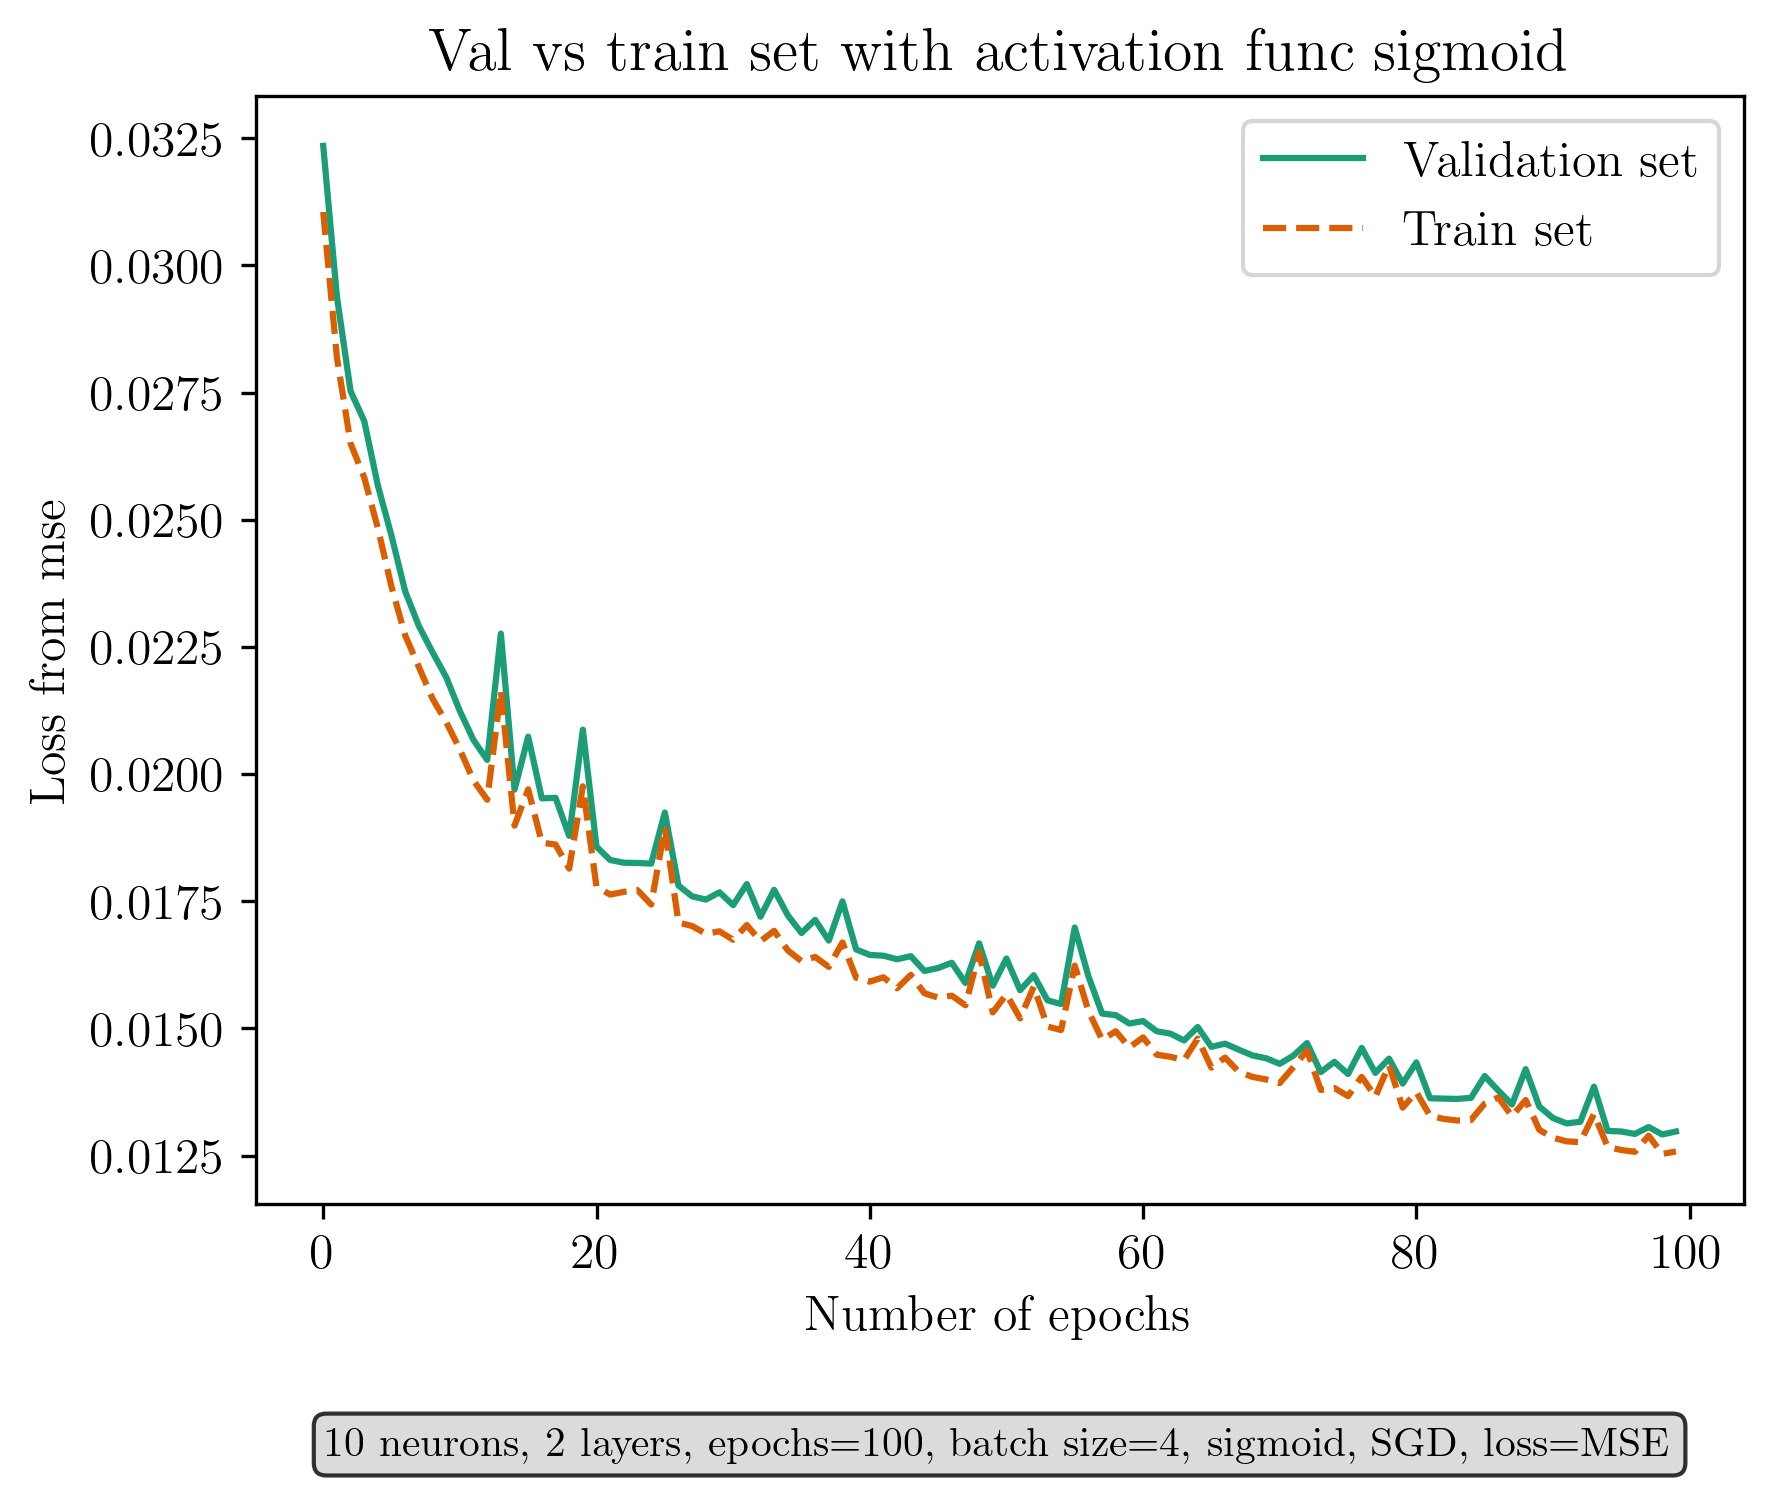
\includegraphics[width=\textwidth]{figures_franke/mse_val_vs_train_sigmoid.png}
        \end{minipage}
        \hfill
        \begin{minipage}{0.325\textwidth}
            \centering
            \textbf{F2} Bias initializations \label{fig:F2} \\  % Label added
            \includegraphics[width=\textwidth]{figures_franke/bias_initialization_franke_minimal.png}
        \end{minipage}
        \begin{minipage}{0.325\textwidth}
            \centering
            \textbf{F3} LR vs batch sizes (fixed)\label{fig:F3} \\  % Label added
            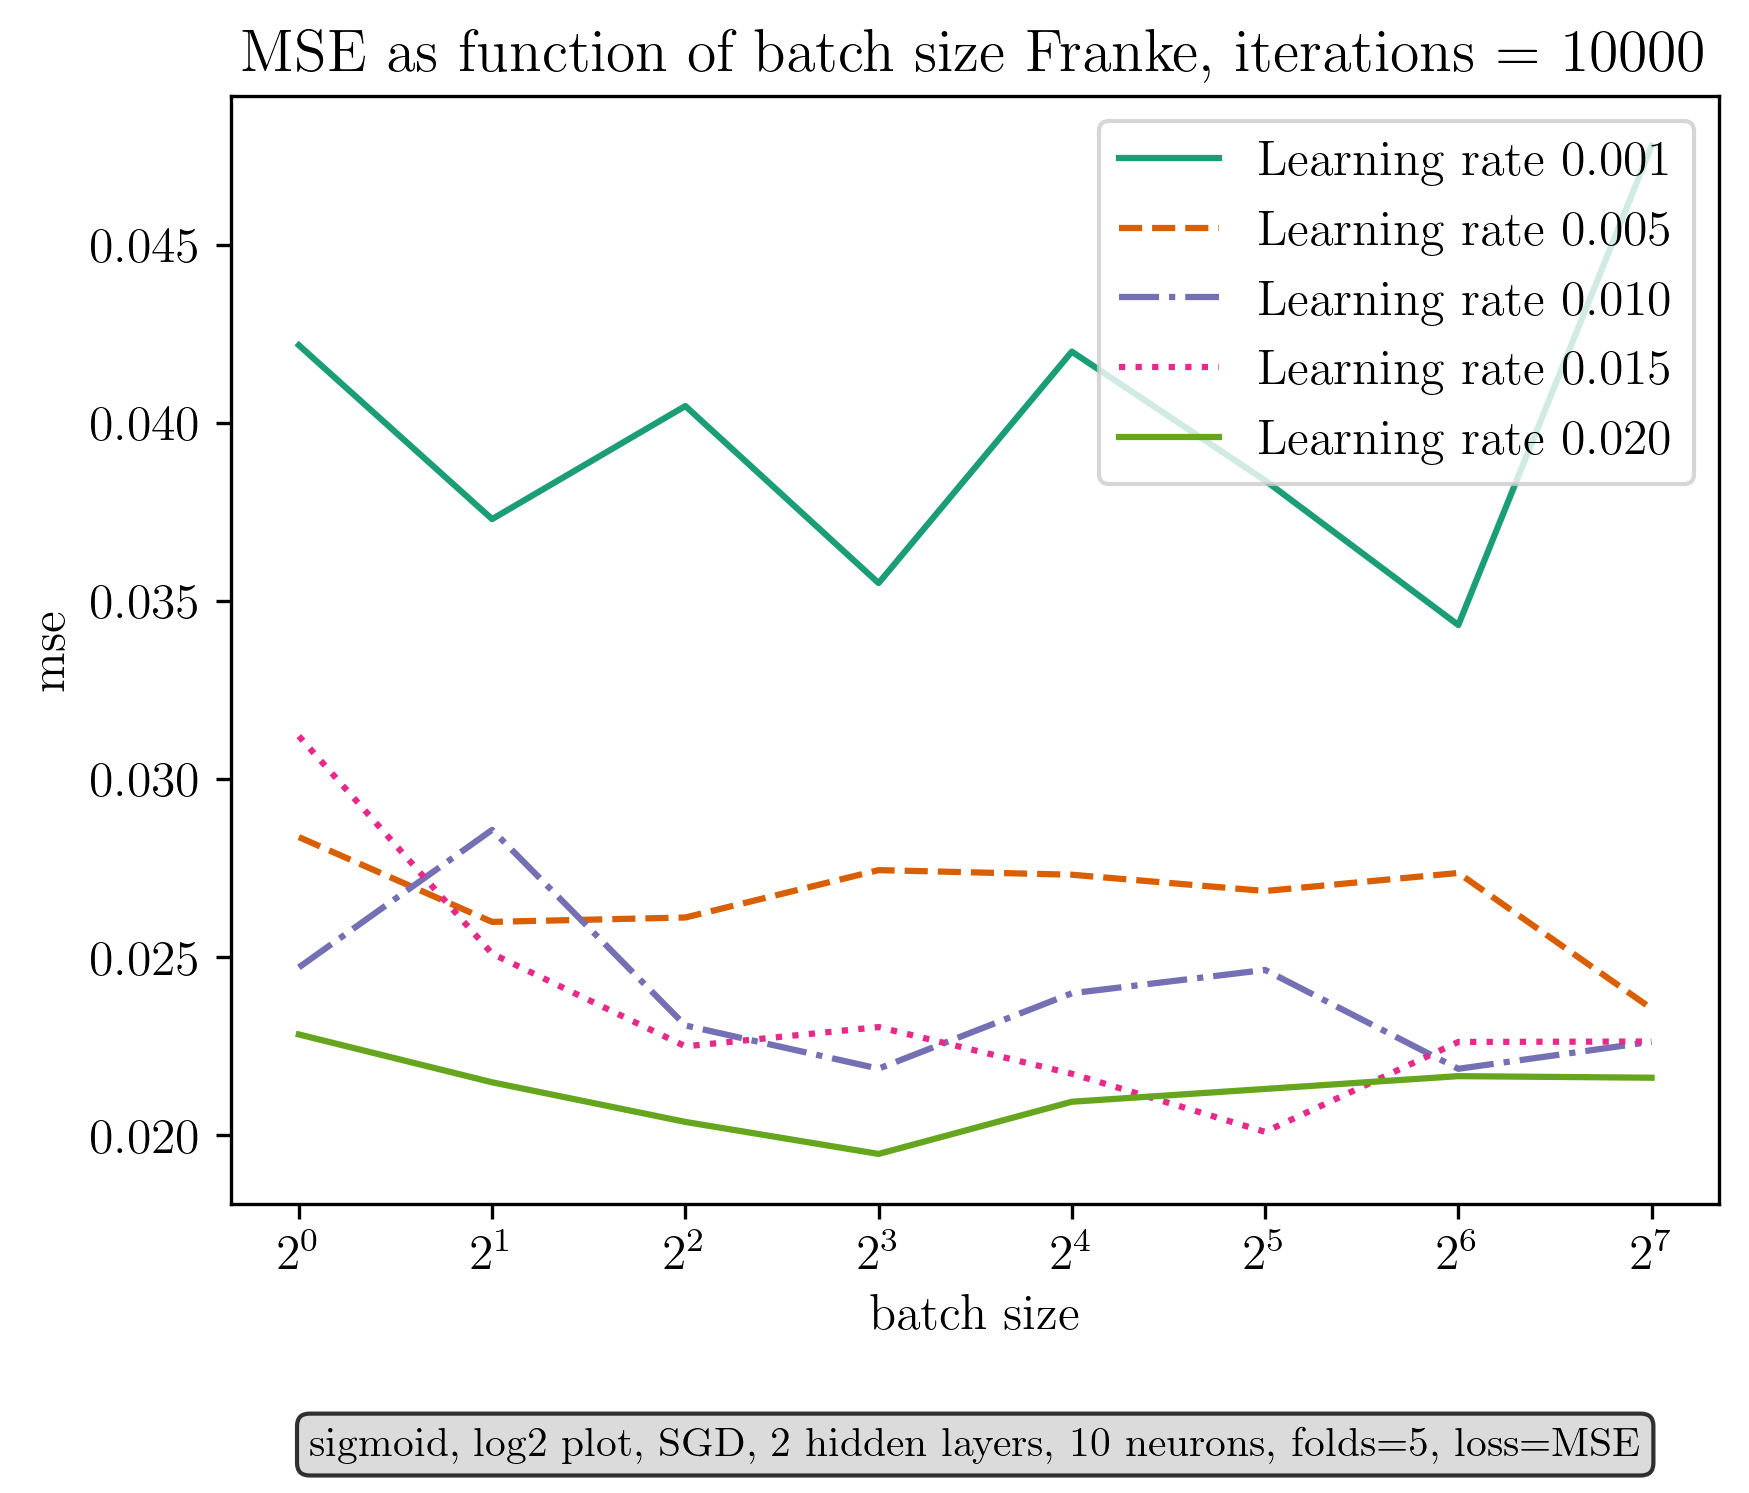
\includegraphics[width=\textwidth]{figures_franke/mse_learning_rate_batch_size_sigmoid_fixed_iterations.png}
        \end{minipage}
        \begin{minipage}{0.325\textwidth}
            \centering
            \textbf{F4} Time usage (fixed iterations) \label{fig:F4} \\  % Label added
            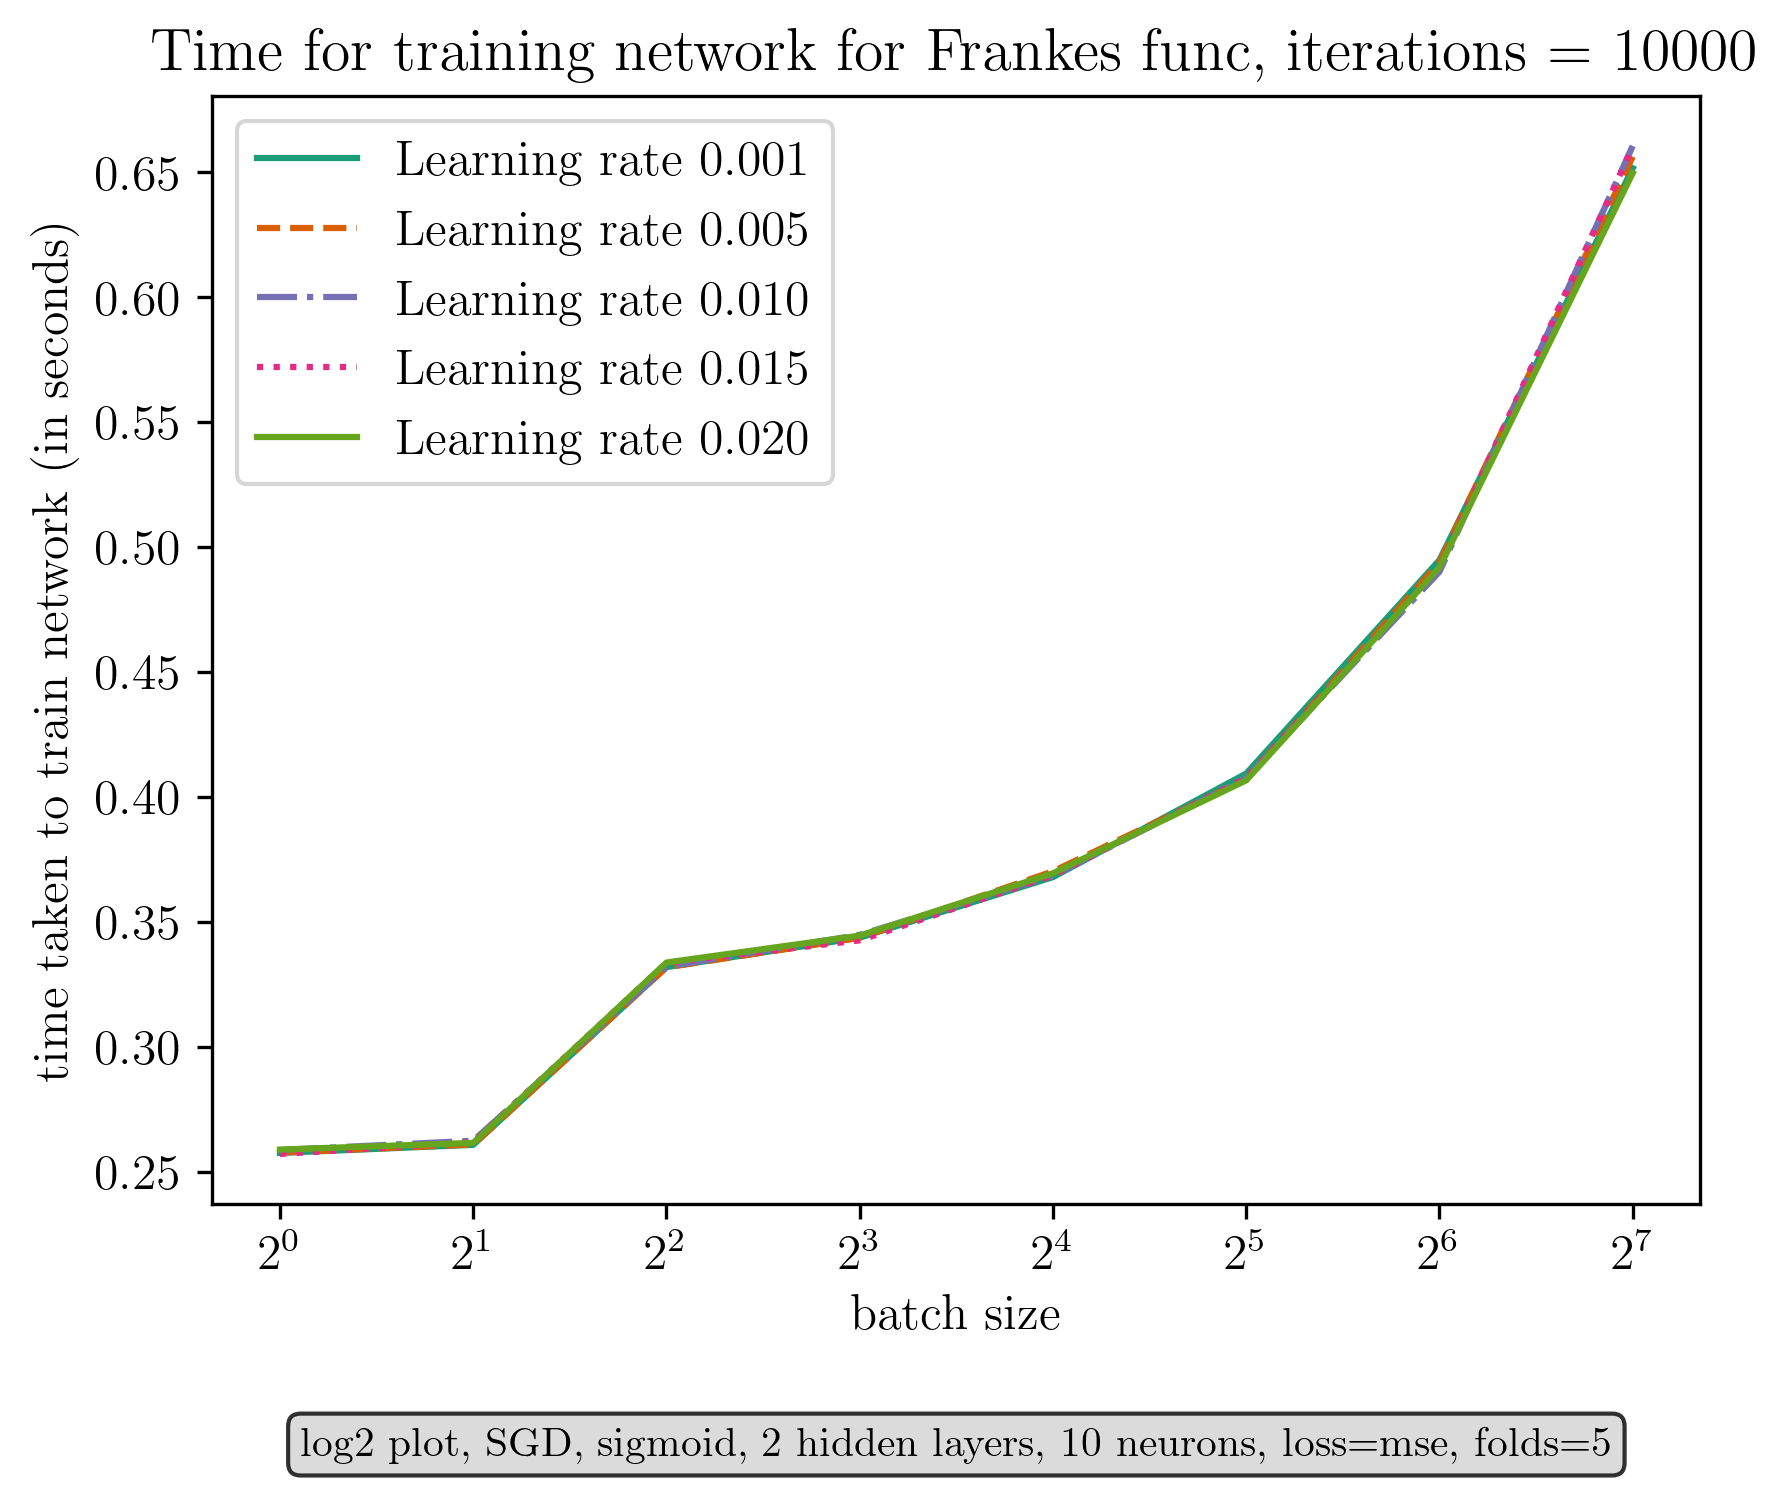
\includegraphics[width=\textwidth]{figures_franke/time_given_batchsize_fixed_iterations_frankes.png}
        \end{minipage}
        \begin{minipage}{0.325\textwidth}
            \centering
            \textbf{F5} MSE vs number of layers \label{fig:F5} \\  % Label added
            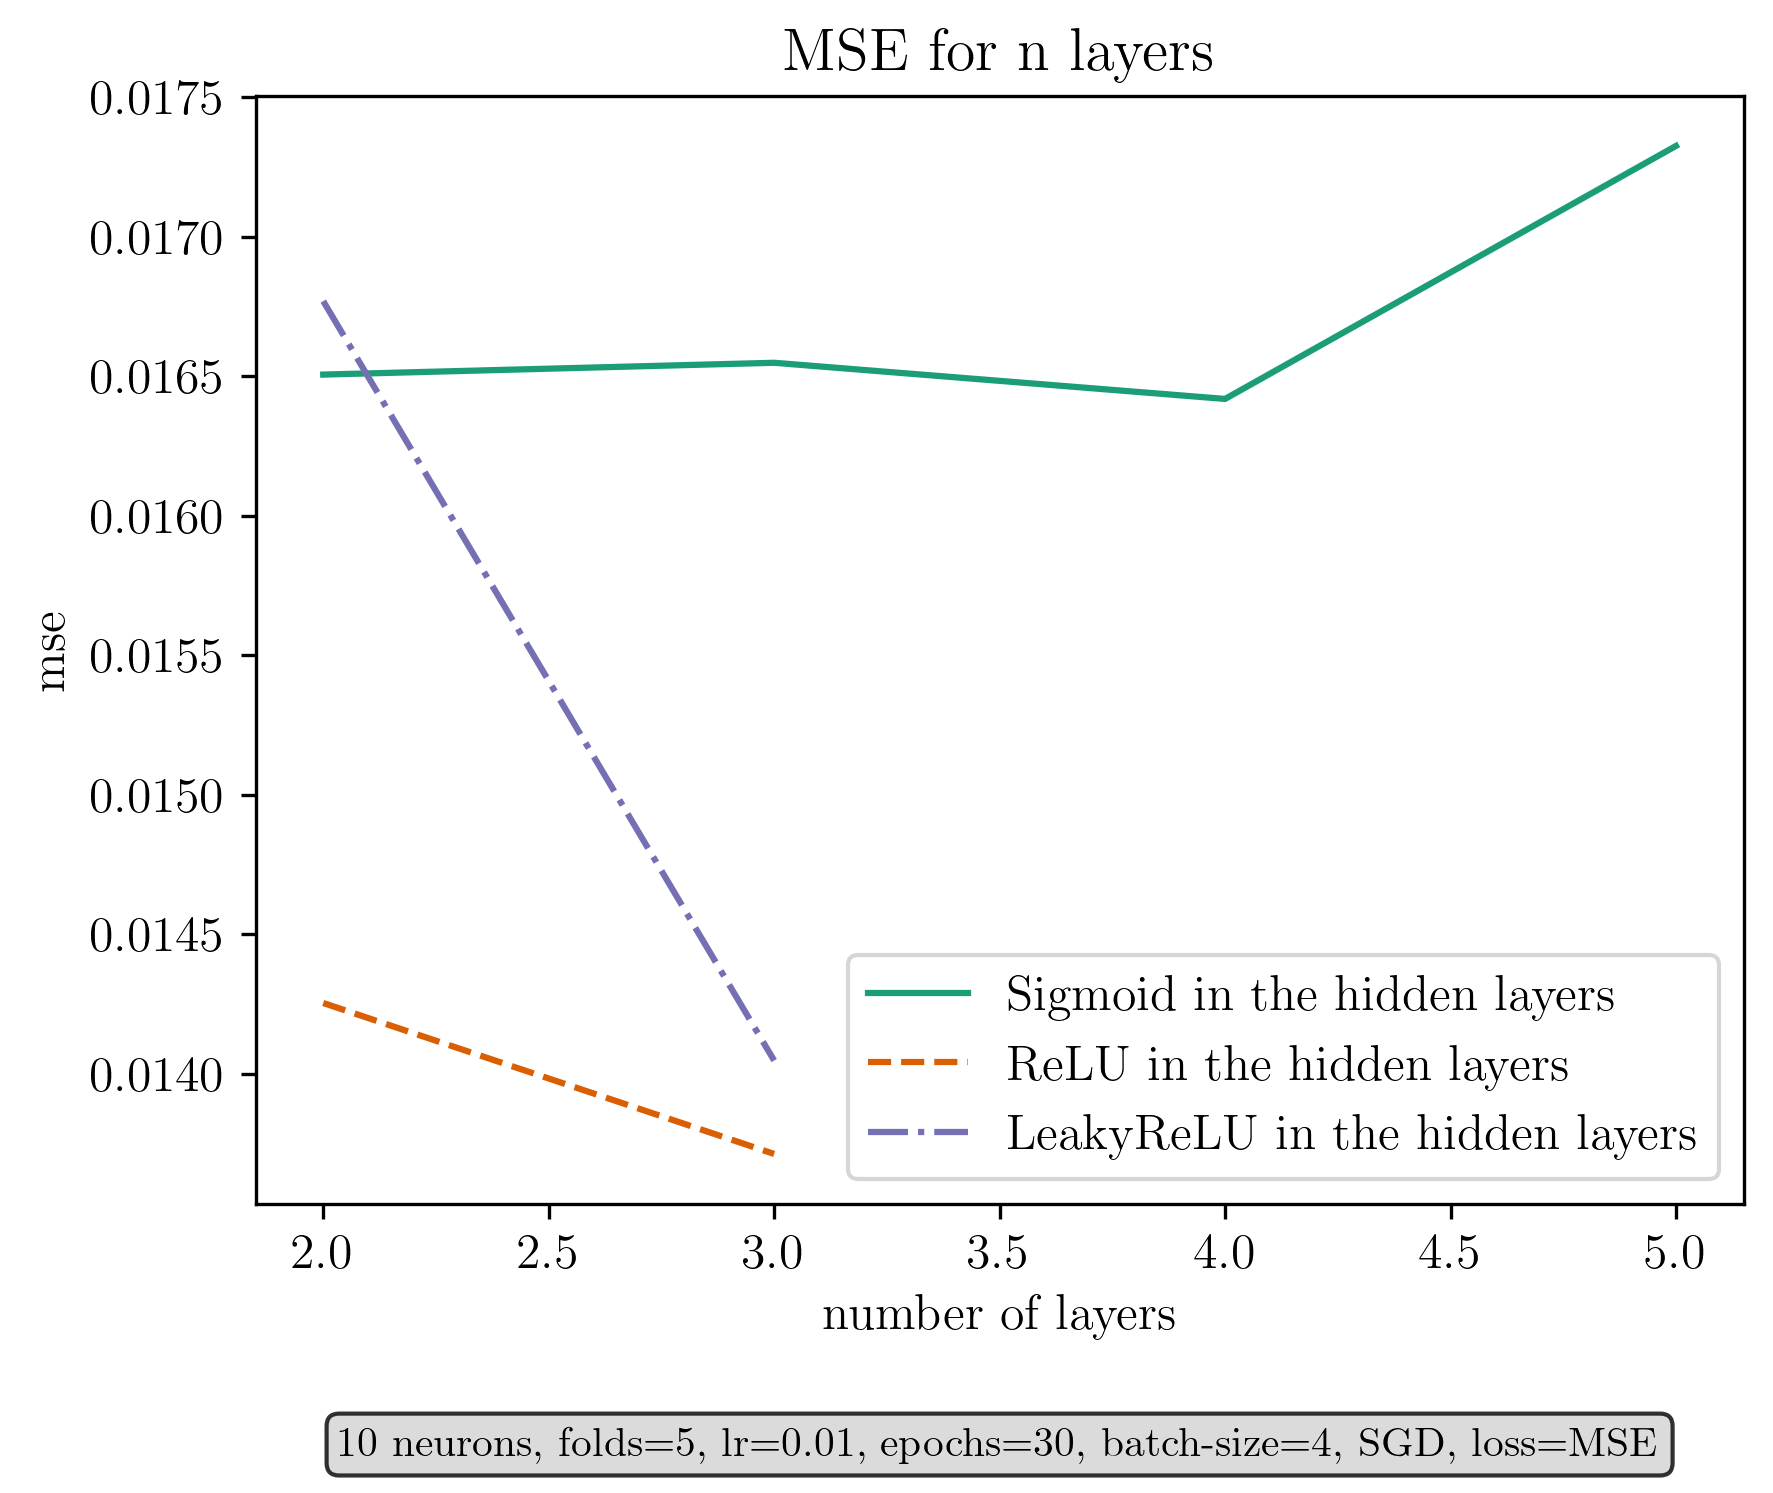
\includegraphics[width=\textwidth]{figures_franke/mse_n_hidden_layers_franke.png}
        \end{minipage}
        \begin{minipage}{0.325\textwidth}
            \centering
            \textbf{F6} MSE vs number of parameters \label{fig:F6} \\  % Label added
            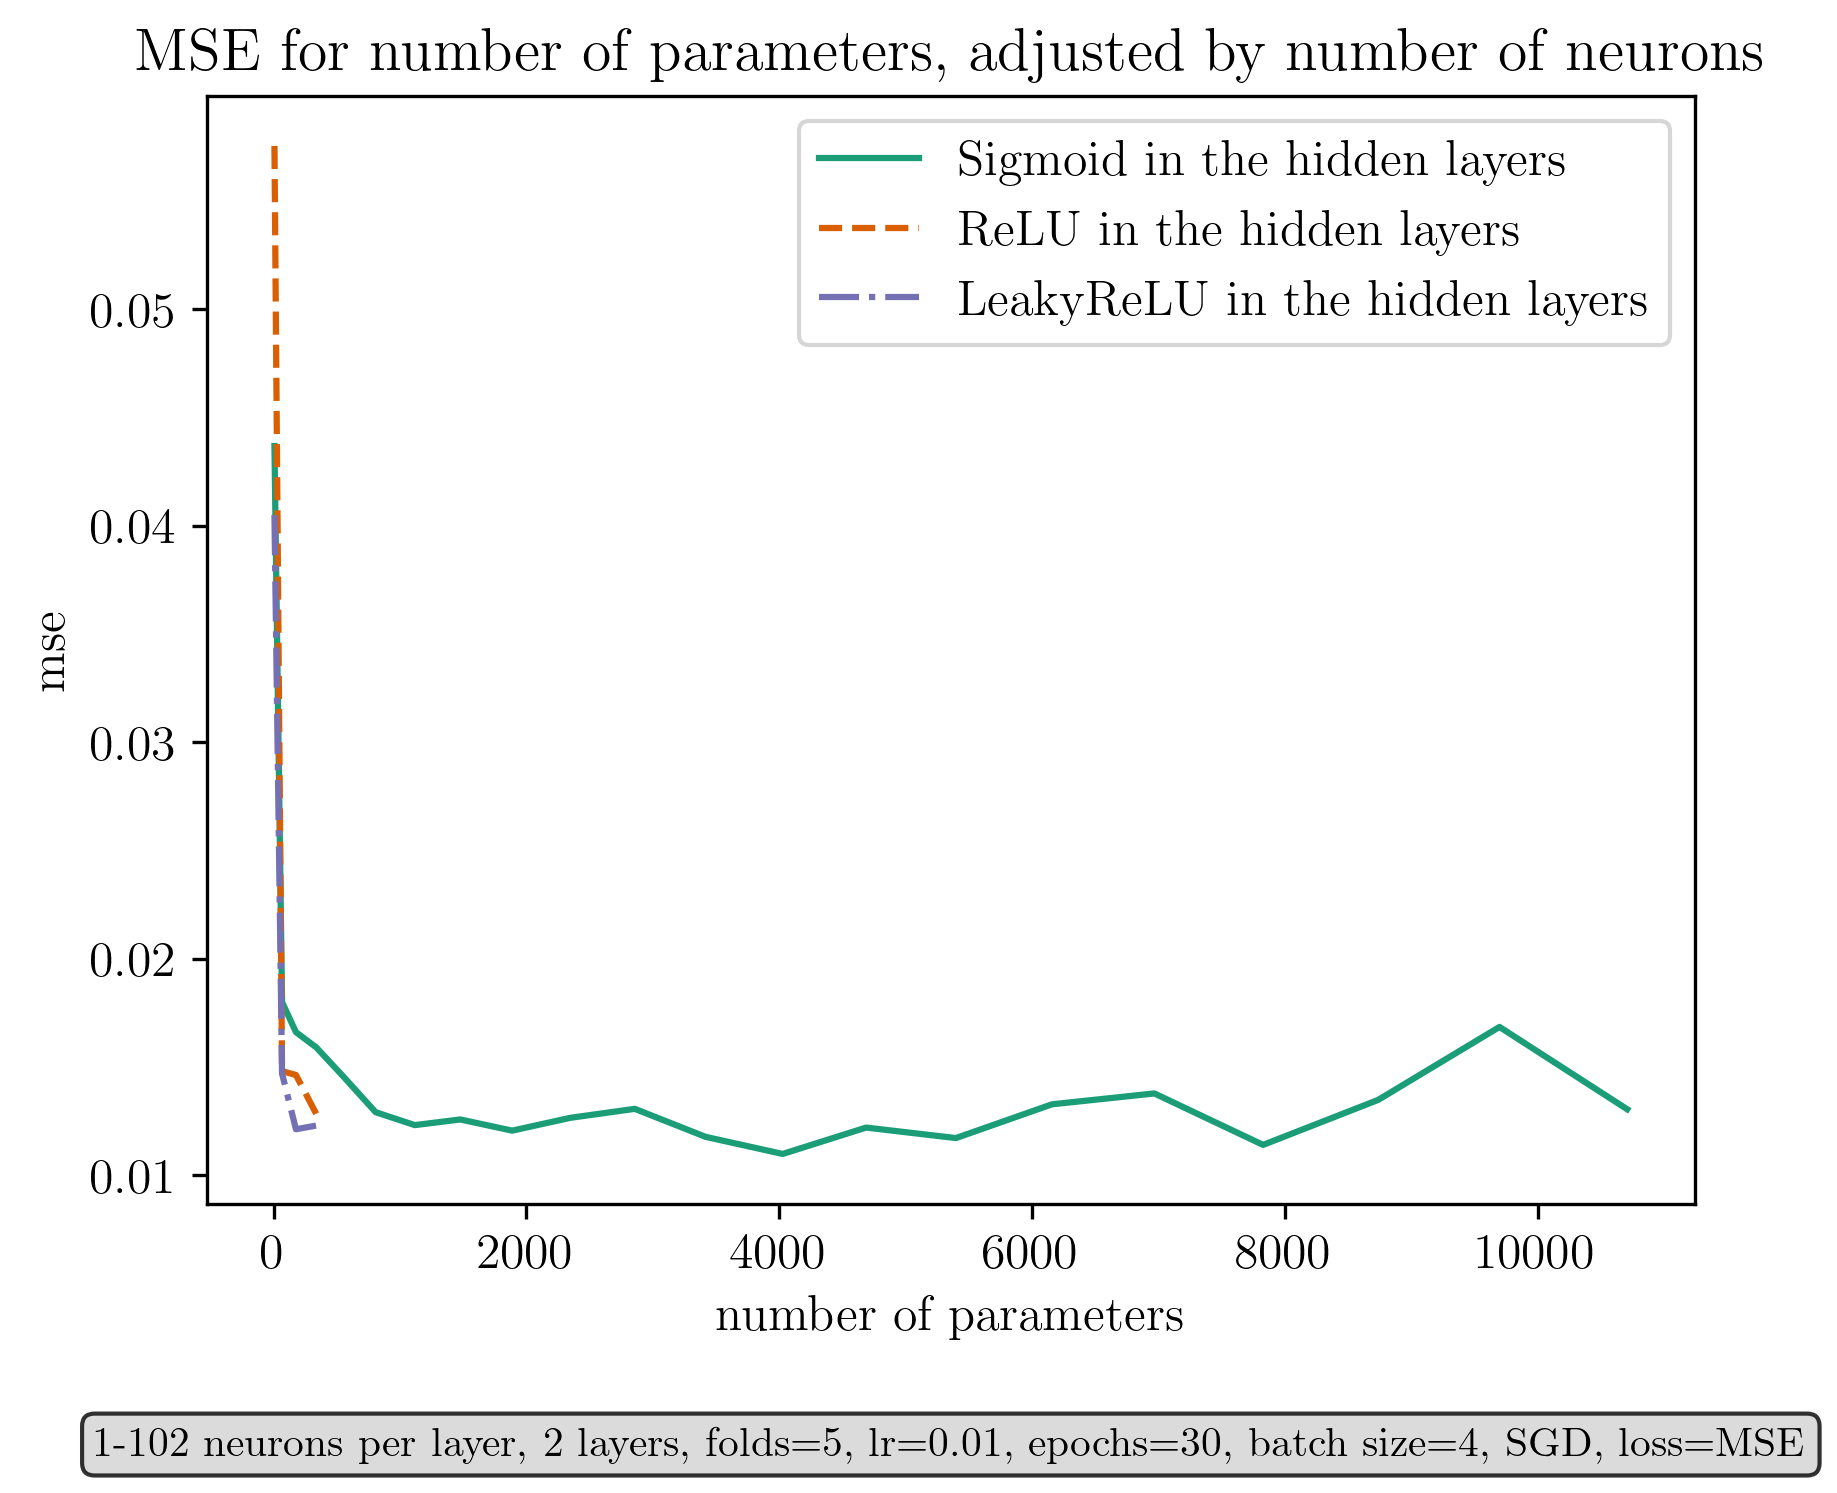
\includegraphics[width=\textwidth]{figures_franke/mse_n_neurons_franke.png}
        \end{minipage}
        \hfill
        \begin{minipage}{0.325\textwidth}
            \centering
            \textbf{F7} MSE for varying $\lambda$, \eta\label{fig:F7} \\  % Label added
            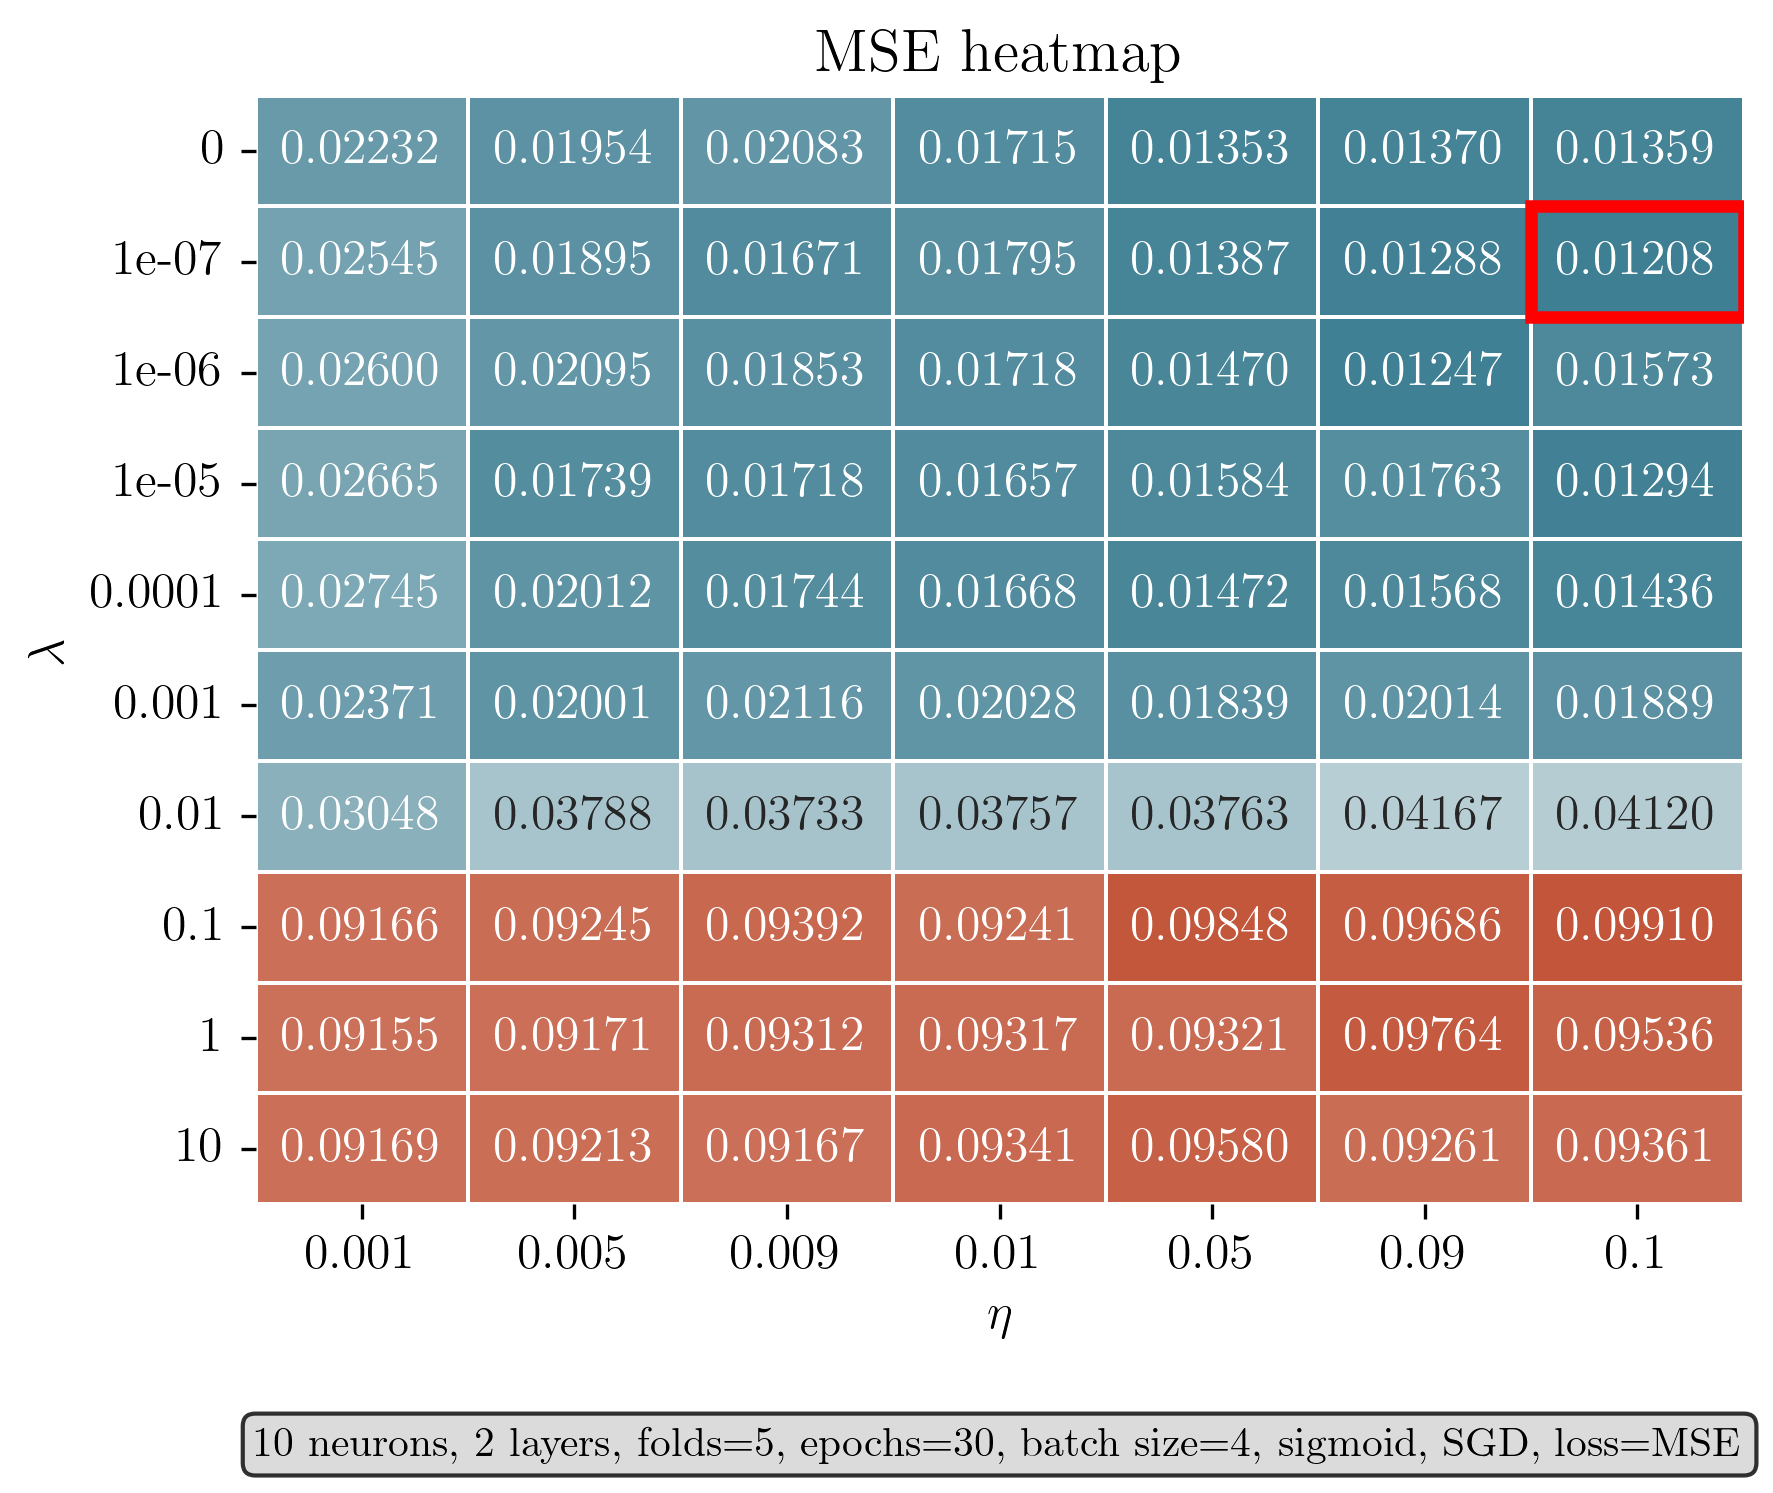
\includegraphics[width=\textwidth]{figures_franke/mse_heatmap_lambda_lr_franke.png}
        \end{minipage}
        \begin{minipage}{0.325\textwidth}
            \centering
            \textbf{F8} Custom NN vs PyTorch\label{fig:F8} \\  
            % Label added
            \includegraphics[width=\textwidth]{figures_franke/franke_custom_vs_torch.png}
        \end{minipage}
            \begin{minipage}{0.325\textwidth}
            \centering
            \textbf{F9} 3D-plot of prediction\label{fig:F9} \\  % Label added
            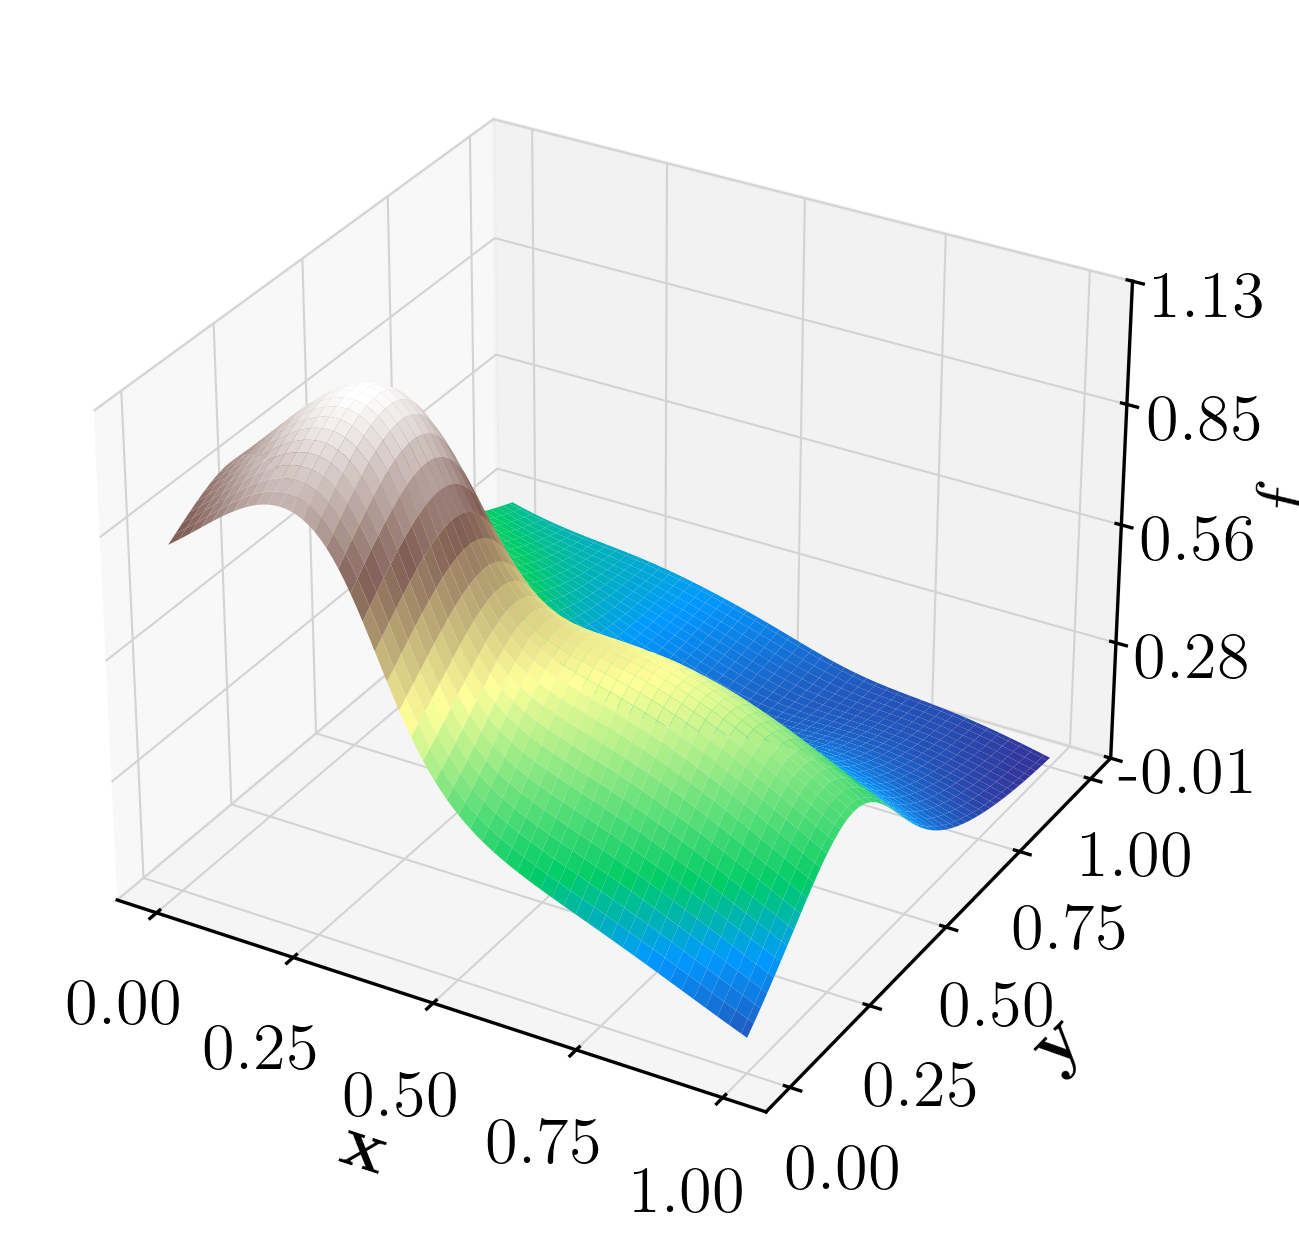
\includegraphics[width=\textwidth]{figures_franke/franke_nn_3d.png}
        \end{minipage}
    
        \vspace{1em}
        \caption*{\textbf{Testing FFNN with Franke’s function: }
        \textbf{F1} MSE over epochs. 2 hidden layers with 10 neurons. Sigmoid activations. Epochs: 100, lr: 0.01, batch size: 4, optimizer: SGD, loss: MSE. 
        \textbf{F2} Different bias initializations. 2 hidden layers with 10 neurons, and Sigmoid activations. $k$ folds with $k=5$. Epochs: 30, lr: 0.01, batch size: 4, optimizer: SGD, loss: MSE. 
        \textbf{F3} $\log_2$-plot of learning rates vs. batch sizes for fixed iterations ($i = 10000$). 2 hidden layers with 10 neurons, and sigmoid activations. $k$ folds with $k=5$. Learning rate: 0.01, optimizer: SGD, loss: MSE. 
        \textbf{F4} $\log_2$-plot of time usage vs. batch size for fixed iterations ($i = 10000$). 2 hidden layers with 10 neurons, and sigmoid activations. $k$ folds with $k=5$. Loss function: MSE. 
        \textbf{F5} MSE vs. number of layers. 10 neurons in each layer. $k$ folds with $k=5$. Epochs: 30, lr: 0.01, batch size: 4, optimizer: SGD, loss: MSE. The plot clearly shows how the ReLU and LeakyReLU activation functions collapse for a number of layers larger than 3. 
        \textbf{F6} MSE vs. number of parameters. 2 hidden layers with 10 neurons. $k$ folds with $k=5$. Epochs: 30, lr: 0.01, batch size: 4, optimizer: SGD, loss: MSE. Similarly, the ReLU and LeakyReLU activation functions fail when the total network size (number of parameters) grows larger, while Sigmoid holds. 
        \textbf{F7} Heat plot of MSE given varying regularization terms $\lambda$ and varying learning rate $\eta$. 2 hidden layers with 10 neurons. $k$ folds with $k=5$. Epochs: 30, batch size: 4, optimizer: SGD, loss: MSE.  
        \textbf{F8} Plot showing how our custom-built FFNN benchmarks against PyTorch. Custom NN: 2 hidden layers with 10 neurons. $k$ folds with $k=5$. Epochs: 5, lr: 0.01, batch size: 4, optimizer: SGD, loss: MSE. PyTorch trained similarly. Note that the weights have been initialized manually using \texttt{torch.nn.init.normal} with \texttt{mean=0.0, std=1.0}.
        \textbf{F9} Final prediction by our custom NN. 2 hidden layers with 10 neurons and sigmoids. Epochs: 30, lr: 0.01, batch size: 4, optimizer: SGD, loss: MSE, $\lambda$ = 1e-7}
        \label{fig:franke_figs}
    \end{minipage}
    }
\end{figure}
\restoregeometry

\newpage
\restoregeometry
\section*{Testing the Breast Cancer Wisconsin (Diagnostic) dataset}

\begin{multicols}{2}

With our neural network now producing satisfactory results for Franke's Function data, we will switch to a classification problem. Specifically, we will fine-tune our network for the \textbf{Breast Cancer Wisconsin (Diagnostic) dataset}. We start off by exploring which insights transfer well from our findings with Franke's Function, and gradually move over to more specific tuning of the Breast Cancer dataset. As with Franke's Function, we will resample with cross validation.

\subsection*{Framework for Breast Cancer Wisconsin (Diagnostic)}
Initially, we reproduce the bias initialization plot for this dataset. (please refer to the \href{https://github.com/EOH-ML/FYS-STK3155-Projects/tree/main/project2}{\texttt{repository}} for plots).  We generally observe the same results as for Franke's Function, namely that if we initialize around $0$, the effect on the performance is negligible. Therefore, we will continue to initialize biases using a standard normal distibution. 

In our analysis, we also run preliminary testing with various optimization algorithms. As noted by Goodfellow, often the most effective optimizer is the one you are most familiar with \cite{goodfellow_deep_2016}. Thus, partly arbitrary, we choose to concentrate on the RMSProp algorithm for this breast cancer classification problem. RMSProp involves two hyperparameters, which is less than Adam and more than SGD. We suggest that this strikes a good balance for our further analysis. 

For the inital testing, we look at number of parameters for different activation functions (SGD in figure \hyperref[fig:BC1]{\textbf{BC1}} and RMSProp in figure \hyperref[fig:BC2]{\textbf{BC2}}). Without any fine-tuning, RMSProp demonstrates promising performance. Based on the insights from figure \hyperref[fig:BC2]{\textbf{BC2}}, we propose using the sigmoid activation function, as it appears to work well in combination with RMSProp for this classification task. For the output layer, we use  the softmax activation function.  We also observe that two hidden layers with 32 neurons each, seem to produce robust results, this is also demonstrated in figure \hyperref[fig:BC3]{\textbf{BC3}}.

When choosing the batch size, we generally observe similar patterns to those found with Franke's Function. (again, please refer to the \href{https://github.com/EOH-ML/FYS-STK3155-Projects/tree/main/project2}{\texttt{repository}} for plots) Specifically, a $\text{batch size} \leq 2^3$ proves beneficial, as it significantly reduces runtime while still yielding high-accuracy results. This assumes that we adjust the number of epochs to achieve a target number of iterations (Equation \ref{eq:epochs_iterations_batch_sample}).

\subsection*{Tuning RMSProp}
With our general framework now in place for this dataset, we are prepared to delve into fine-tuning specific parameters within the RMSProp algorithm.

As a starting point, we create a heat map (Figure \hyperref[fig:BC4]{\textbf{BC4}}) with learning rates along the x-axis, decay rates along the y-axis, and the accuracy of the validation set for each combination. We find that a learning rate of $0.01$ combined with a decay rate of $0.9$ maximizes accuracy at $0.9802$.

To further strengthen our analysis, we now explore the effects of an added L2-regularization term $\lambda$. The impact of this, in combination with a varying learning rates, can be studied in figure \hyperref[fig:BC5]{\textbf{BC5}}. It is difficult to provide one general take-away, as regularization sometimes proves beneficial, and sometimes not. For the combination that maximizes the accuracy, we have a regularization of $\lambda = 10^{-7}$. Therefore, as with Franke's Function, we suggest exploring the effect of a regularization term, as it can sometimes increase accuracy.

Once again, we note that these findings are not absolute, and more thourough analysis of these parameters in combination with the previously discussed parameters could provide an even better accuracy. 

Based on our finds, we recommend using RMSProp with a learning rate of $0.05$, a regularization term of $10^{-7}$, and a decay rate of 0.9. The network setup includes two hidden layers with 32 neurons each, using sigmoid activation, a batch size of $4$, and $30$ epochs. This configuration tends to yield a well-trained neural network for the Breast Cancer Wisconsin (Diagnostic) dataset. The resulting predictions produce the confusion matrix shown in Figure \hyperref[fig:BC6]{\textbf{BC6}}.

Our intuition is that further analysis with Bayes' formula on this result could provide some additional insights, however time constraints limit us from doing so.

\subsubsection*{Testing with Logistic Regression}
When applying logisitic regression to predict cancer diagnoses, our goal is to identify a set of parameters that maximize accuracy. We implement a logistic regression model using Stochastic Gradient Descent, with a scheduled learning optimizer. \cite{hjorth-jensen_applied_2021} Figure \hyperref[fig:BC7]{\textbf{BC7}} illustrates  that multiple training configurations can yield high validation accuracy. The heatmap displays validation accuracy across various batch sizes and regularization parameters. We find that the results vary across runs, likely due to random parameter initialization, and the tendency of gradient descent to get stuck in local minima. Nevertheless, our primary aim is to acheive a highly accurate model.

We store the five top-performing models and proceed to testing. As shown in Figure \hyperref[fig:BC8]{\textbf{BC8}}, all models achieve high accuracy, with one model standing out as the best. This model will be our final choice.

Finally, we cross-validate our results with Scikit-Learn's own \texttt{SGDClassifier}, which is similar to our logistic regression implementation. From this we obtain similar outcomes.

\subsection*{Comparison of FFNN with Logistic regression}
We are now prepared to compare our logistic regression analysis with the neural network implementation. 
\begin{table}[H]
\centering
\begin{tabular}{|l|c|c|}
\hline
\textbf{Dataset} & \textbf{FFNN} & \textbf{Logistic} \\
\hline
BCW (Acc.) & 0.9824 \hyperref[fig:BC5]{[BC5]} & 0.991 \hyperref[fig:BC8]{[BC8]}\\
\hline
\end{tabular}
\caption{Comparing the results of our feed forward network and the logistic regression model}
\label{tab:table2}
\end{table}

From studying the results in Table \ref{tab:table2}, we see that both logistic regression and the neural network achieve high accuracy on the Breast Cancer Wisconsin (Diagnostic) dataset. The feed-forward neural network may require more fine tuning of hyperparameters, reaching similar accuracy levels when properly optimized. Since logistic regression provides a simpler setup, this would now be our obvious choice. This is on par with our findings with Franke's Function in the previous section.

\subsubsection*{Note on Benchmarking with PyTorch}
For both the approximation and the classification tasks, a PyTorch network is set up with the identical layer depth, activation functions, optimizer, and with the same hyper parameters as our custom networks. Special care is taken in initializing the weights and biases, to ensure that these are normally distributed $\sim \mathcal{N}(0, 1)$, equal to our models. Benchmarking with PyTorch renders only slightly better results (one example is shown in Figure \hyperref[fig:F8]{\textbf{F8}}), and we take this as proof of valid findings from our own implemented model. Please refer to our \href{https://github.com/EOH-ML/FYS-STK3155-Projects/tree/main/project2}{\texttt{repository}} for further plots.
\end{multicols}

\newgeometry{top=1cm, left=1cm, right=1cm}
\begin{figure}[htbp]
    \centering
    \fbox{
    \begin{minipage}{\textwidth}
        \centering
        \begin{minipage}{0.325\textwidth}
            \centering
            \textbf{BC1} Network size, SGD \label{fig:BC1} \\  % Label added
            \includegraphics[width=\textwidth]{figures_wisconsin/SGD_n_neurons_BC_minimal.png}
        \end{minipage}
        \hfill
        \begin{minipage}{0.325\textwidth}
            \centering
            \textbf{BC2} Network size, RMSProp \label{fig:BC2} \\  % Label added
            \includegraphics[width=\textwidth]{figures_wisconsin/RMSProp_n_neurons_BC_minimal.png}
        \end{minipage}
            \begin{minipage}{0.325\textwidth}
            \centering
            \textbf{BC3} Testing ideal network sizes \label{fig:BC3} \\  % Label added
            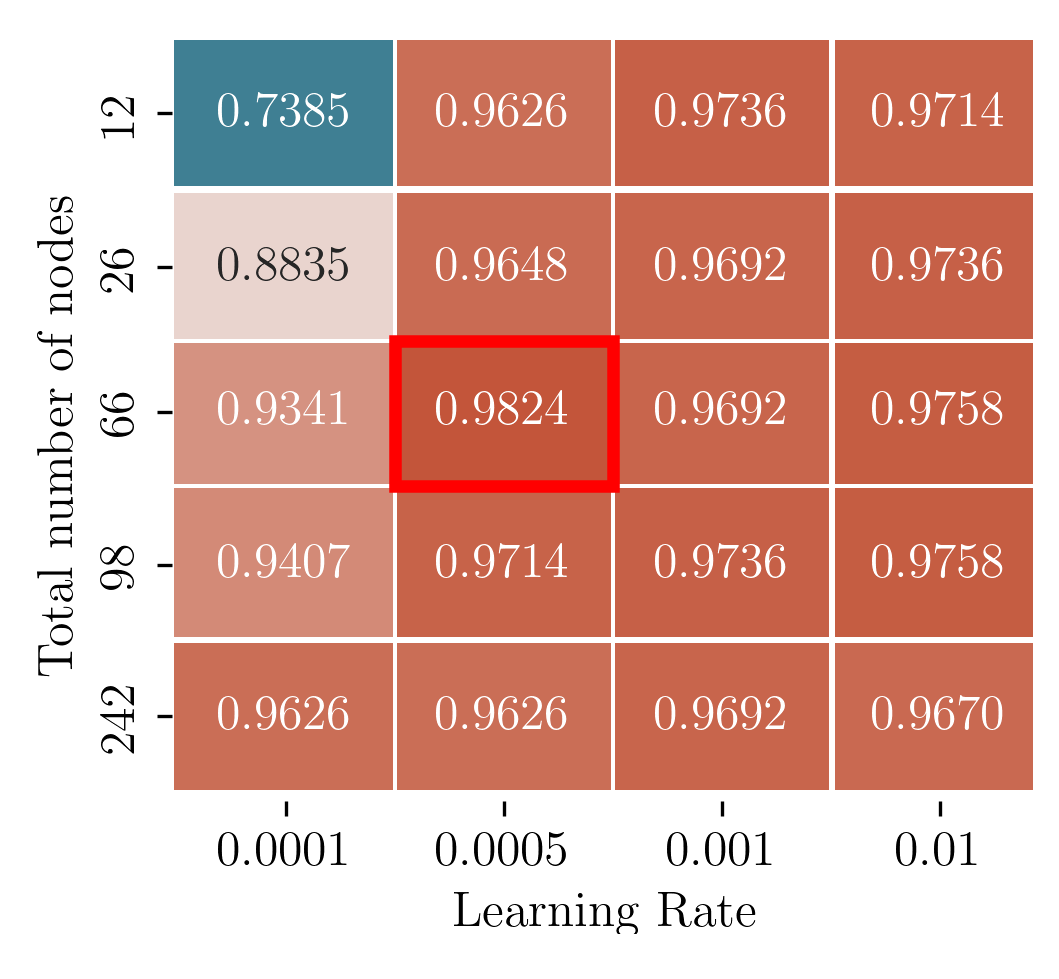
\includegraphics[width=\textwidth]{figures_wisconsin/heatmap_lr_network_size_valid.png}
        \end{minipage}
        \hfill
        \begin{minipage}{0.325\textwidth}
            \centering
            \textbf{BC4} RMSProp: LR vs Decay Rate\label{fig:BC4} \\  % Label added
            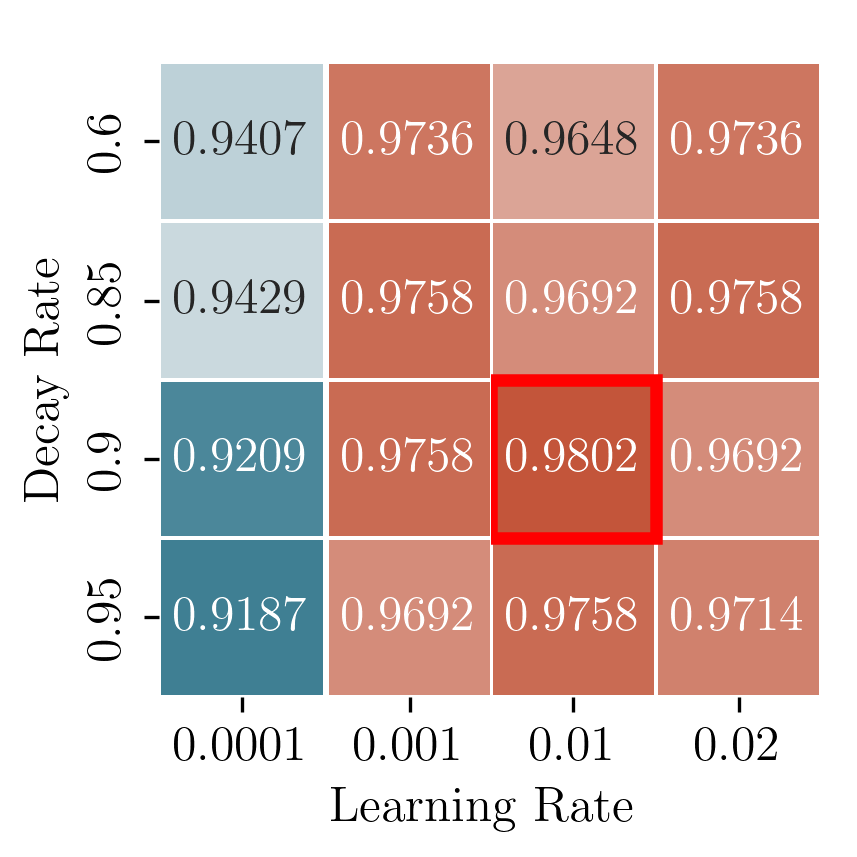
\includegraphics[width=\textwidth]{figures_wisconsin/heatmap_acc_rho_lr_wisconsin.png}
        \end{minipage}
        \begin{minipage}{0.325\textwidth}
            \centering
            \textbf{BC5} RMSProp: $\lambda$ vs $\eta$\label{fig:BC5} \\  % Label added
            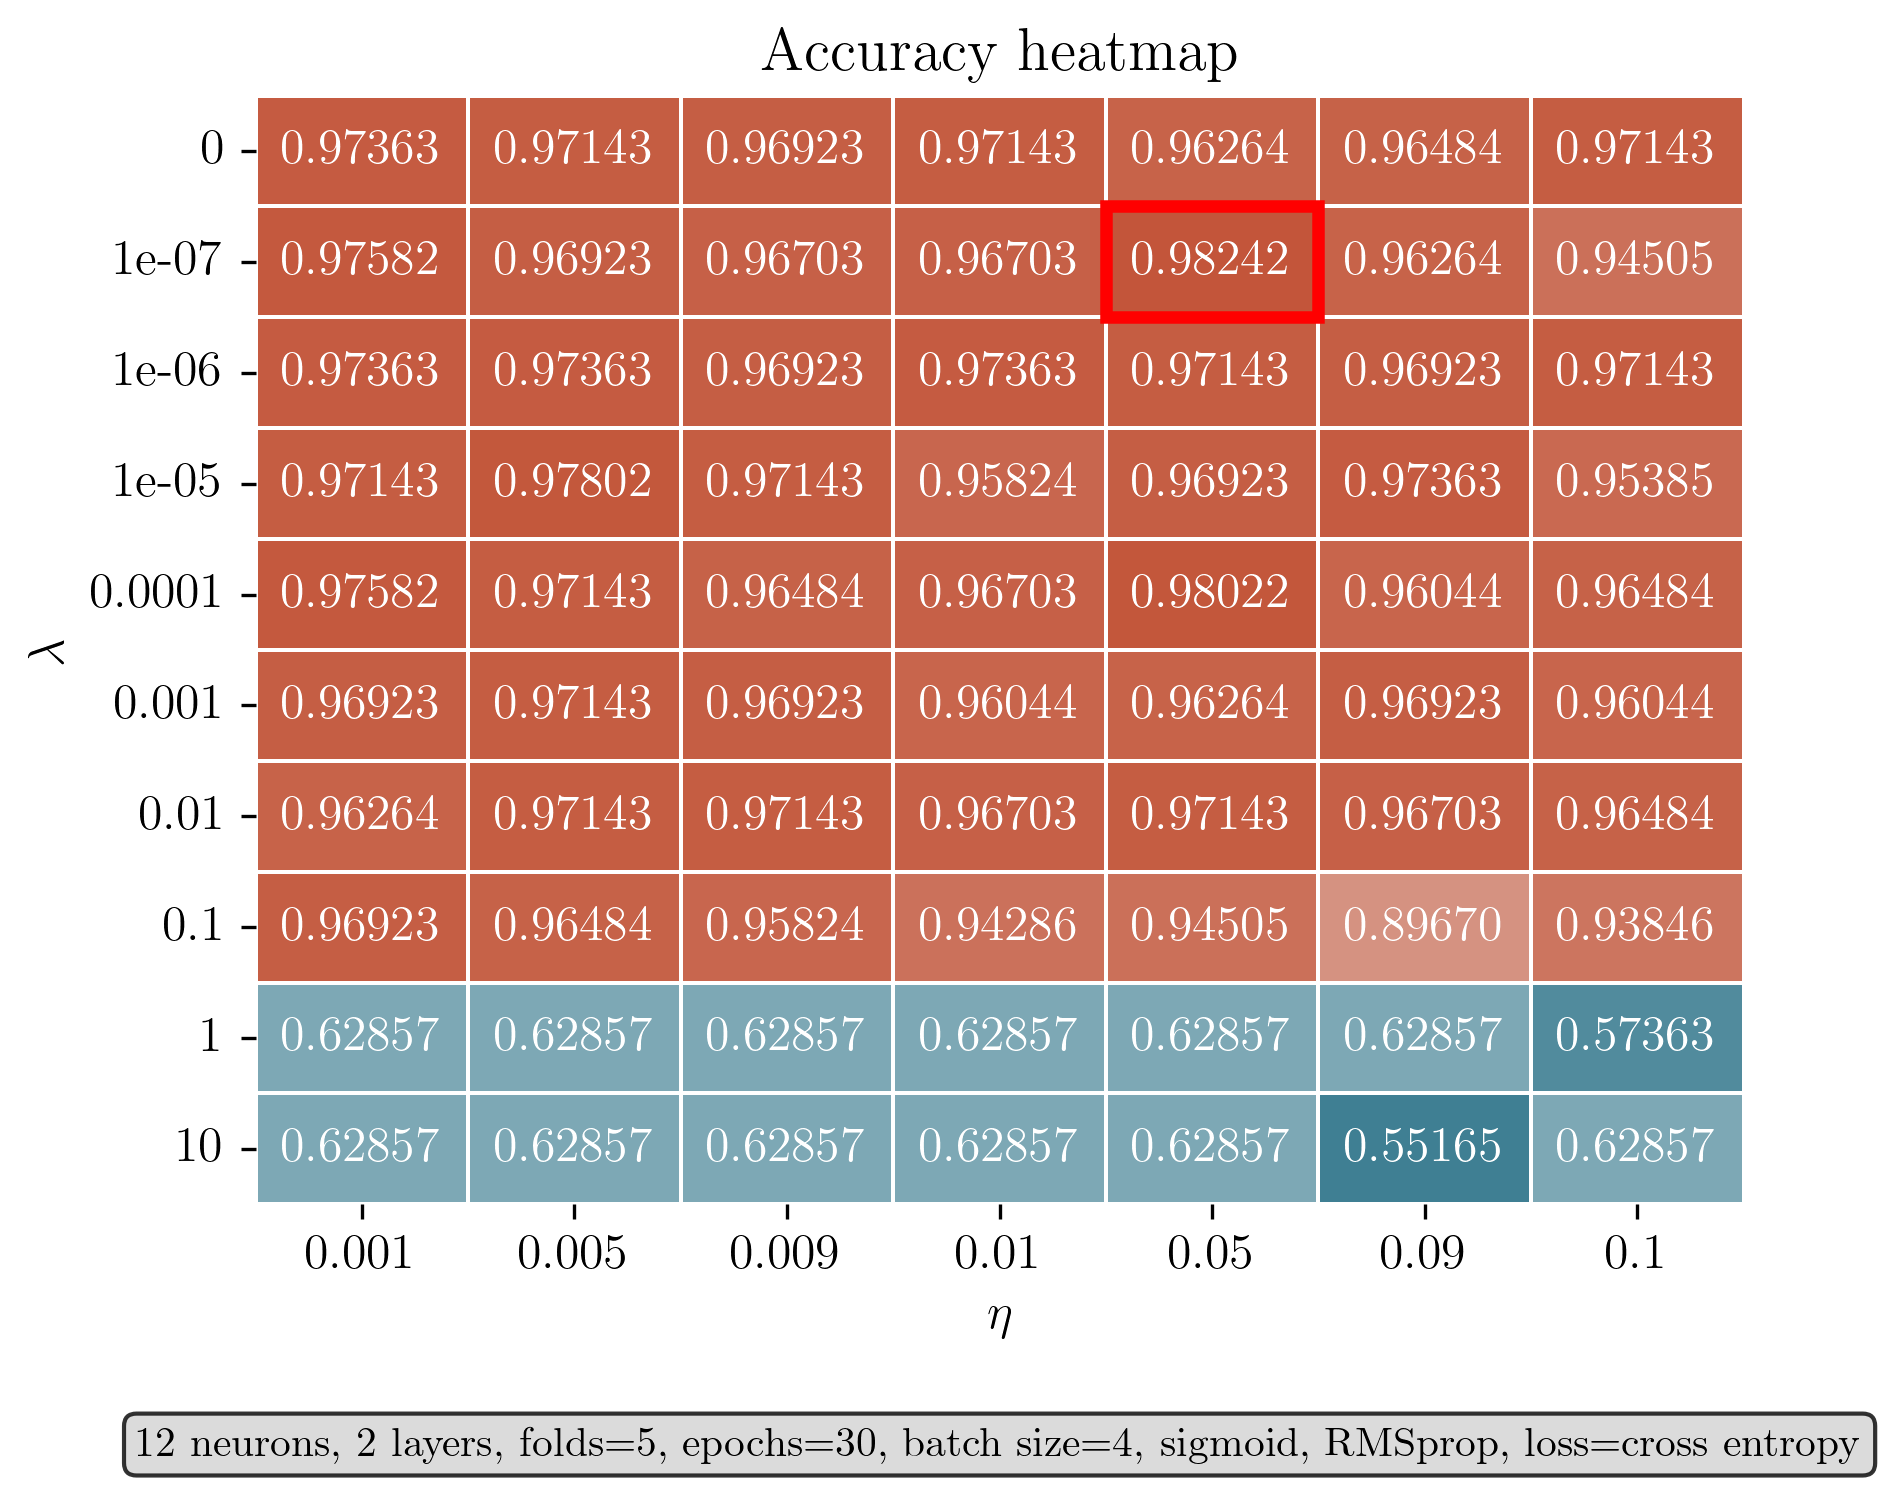
\includegraphics[width=\textwidth]{figures_wisconsin/accuracy_heatmap_lambda_eta_franke.png}
        \end{minipage}
            \begin{minipage}{0.325\textwidth}
            \centering
            \textbf{BC6} Confusion matrix, final model\label{fig:BC6} \\  % Label added
            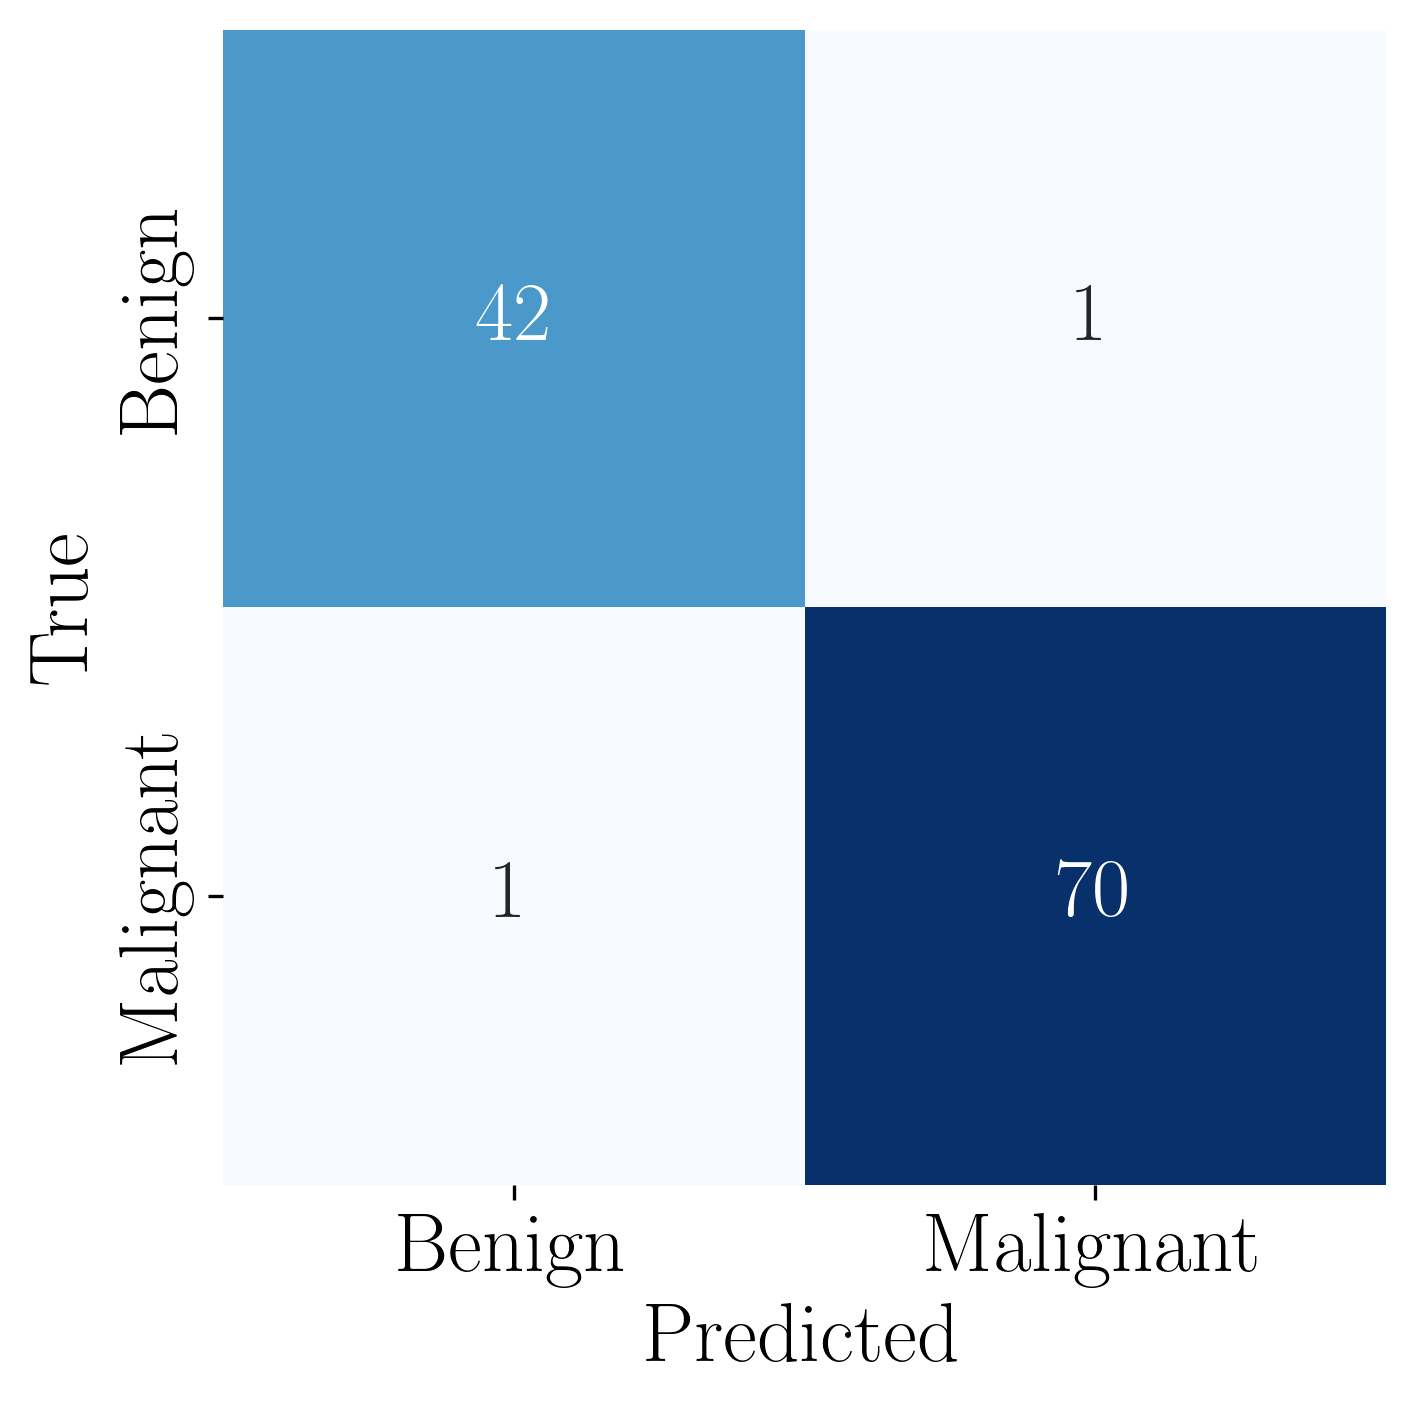
\includegraphics[width=\textwidth]{figures_wisconsin/confusion_matrix_final_model.png}
        \end{minipage}
            \begin{minipage}{0.66\textwidth}
            \centering
            \textbf{BC7} Logistic regression $\lambda$ vs batch size\label{fig:BC7} \\  % Label added
            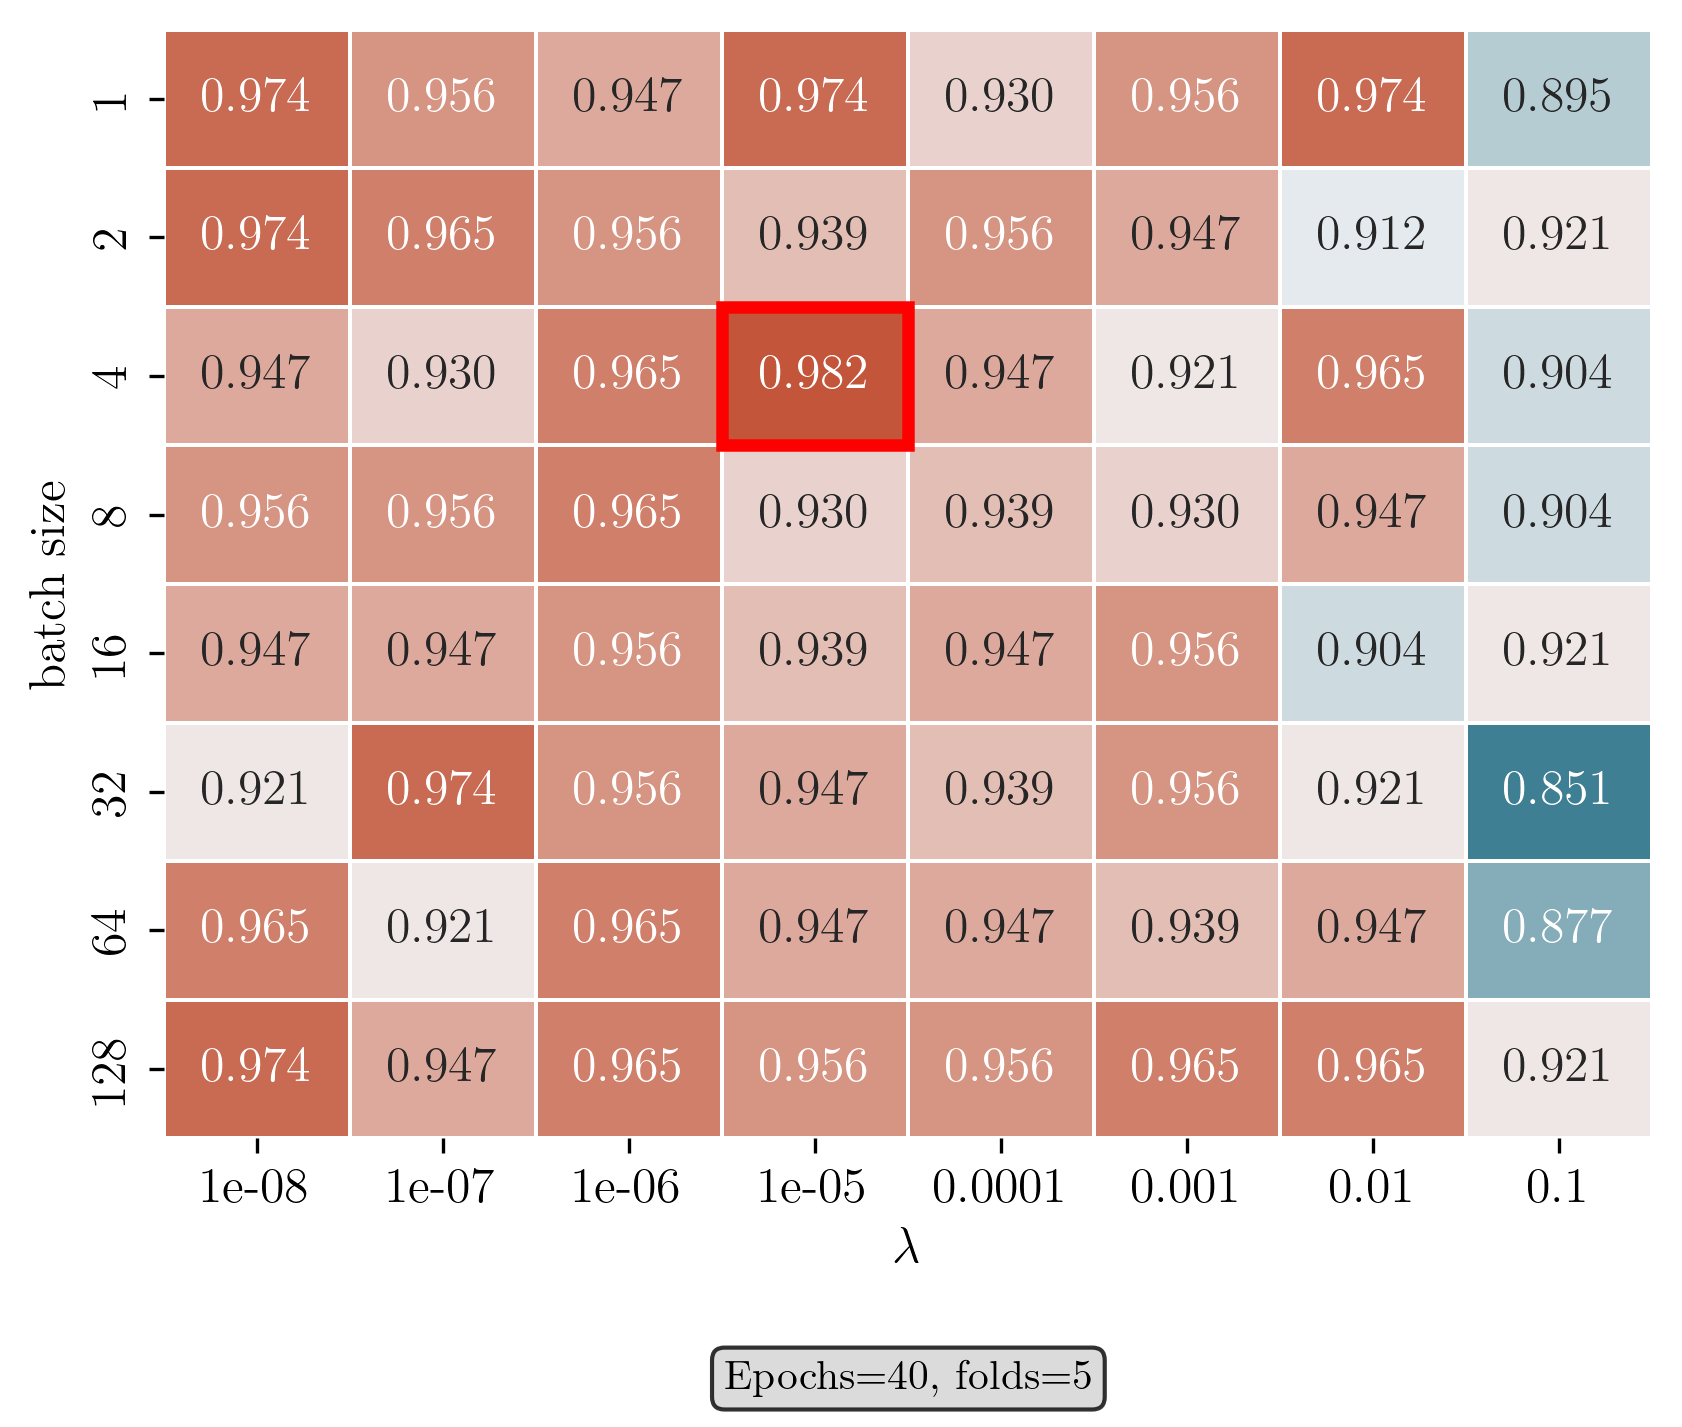
\includegraphics[width=0.85\textwidth]{figures_wisconsin/heatmap_accuracy_batch_size.png}
        \end{minipage}
            \begin{minipage}{0.325\textwidth}
            \centering
            \textbf{BC8} Accuracy, 5 LogReg models \label{fig:BC8} \\ % Label added
            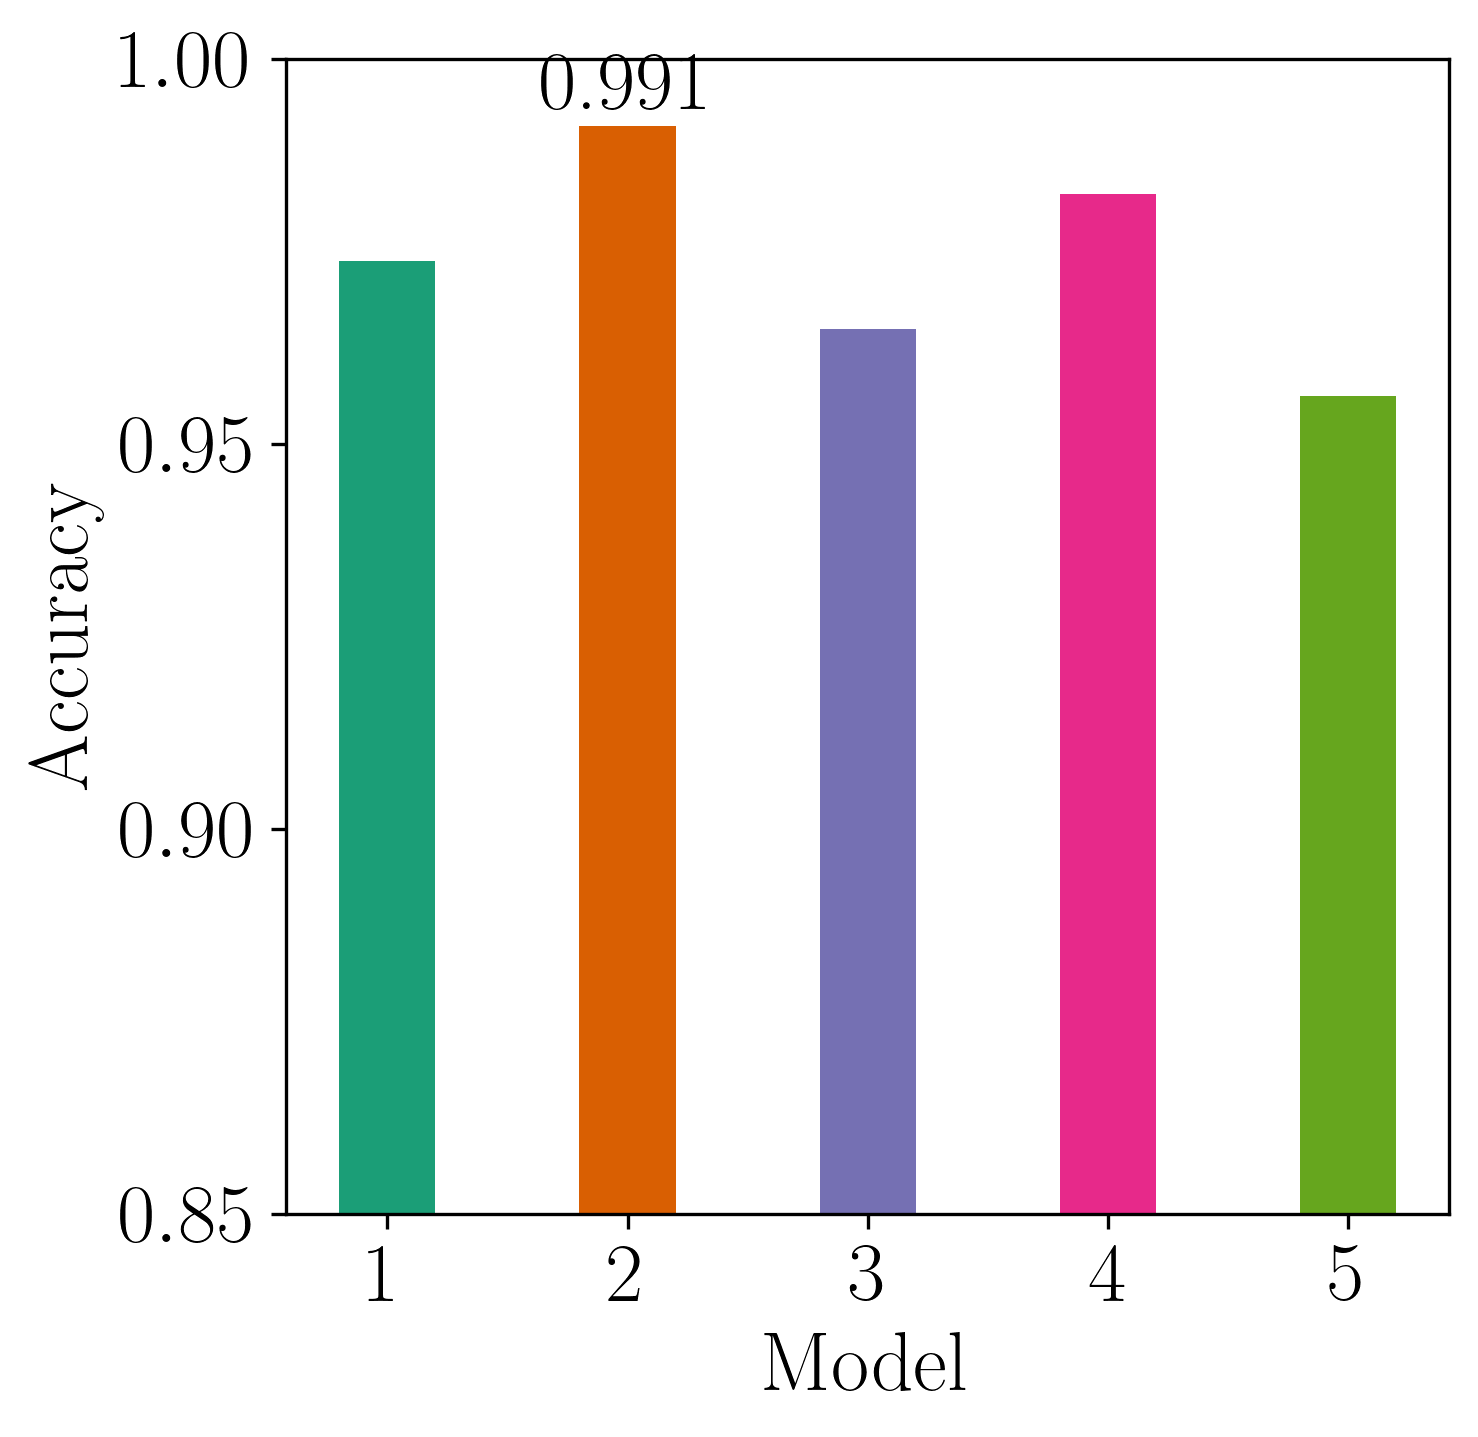
\includegraphics[width=\textwidth]{figures_wisconsin/bars_best_models.png}
        \end{minipage}
        \vspace{0.7em}
        \caption*{\textbf{Testing FFNN with Breast Cancer Wisconsin (Diagnostic) dataset: }\textbf{BC1} Accuracy vs. number of parameters, using SGD optimizer. 2 hidden layers with 32 neurons. Epochs: 30, lr: 0.001, batch size: 4, loss: Cross Entropy Loss. $k$ folds with $k = 5$. 
        \textbf{BC2} Accuracy vs. number of parameters, using RMSProp optimizer. 2 hidden layers with 32 neurons. Epochs: 30, lr: 0.001, $\rho$ = 0.9, batch size: 4, loss: Cross Entropy Loss. $k$ folds with $k = 5$. 
        \textbf{BC3} Testing different network sizes vs learning rates: 12: \texttt{[10, 2]}, 26: \texttt{[16, 8, 2]}, 66: \texttt{[32, 32, 2]}, 98: \texttt{[64, 32, 2]}, 242: \texttt{[128, 64, 32, 16, 2]}. Epochs: 30, batch size: 4, loss: Cross Entropy Loss. $k$ folds with $k = 5$.
        \textbf{BC4} Learning rate vs. tuning of RMSProp's $\rho$ parameter. 2 hidden layers with 32 neurons. Epochs: 30, batch size: 4, loss: Cross Entropy Loss. $k$ folds with $k = 5$. 
        \textbf{BC5} Testing different values of the regularization term $\lambda$ vs. different learning rates ($\eta$).  2 hidden layers with 32 neurons. Epochs: 30, batch size: 4, loss: Cross Entropy Loss. $k$ folds with $k = 5$.
        \textbf{BC6} Confusion matrix for final network, after a prediction run on the test set, resulting in $\text{accuracy}=0.9824$. The labels \textit{Benign} and \textit{Malignant} correspond to \texttt{False}/\texttt{0} and \texttt{True}/\texttt{1} in the dataset. Setup: 2 hidden layers with 32 neurons. Epochs: 30, batch size: 4, lr: 0.01, $\rho$: 0.9, $\lambda$: 1e-7, loss: Cross Entropy Loss.
        \textbf{BC7} Heatmap showing best accuracy based on batch sizes and regularization term $\lambda$. SGD, Cross Entropy Loss, epochs: 40, learning scheduler. \textbf{BC8} Bar plot showing accuracy from independently run Logistic regression models, $n=5$.}
        \label{fig:franke_figs}
    \end{minipage}
    }
\end{figure}
\restoregeometry

\section*{Conclusion}

\begin{multicols}{2}
In this project, we set out to investigate the application of feed-forward neural networks in two different tasks: approximating synthetic data generated from Franke's Function and classifying real medical data from the Breast Cancer Wisconsin (Diagnostic) dataset. After extensive experimentation and model fine-tuning, we achieved strong results in both cases. We then evaluated the performance of our optimized neural networks by comparing them with traditional machine learning techniques: linear regression for Franke's Function, and logistic regression for the breast cancer dataset. This comparison helped us build intuition on the strengths and limitations of each approach.

\begin{table}[H]
\centering
\begin{tabular}{|l|c|c|}
\hline
\textbf{Dataset} & \textbf{FFNN} & \textbf{Log/Lin} \\
\hline
FF (MSE) & 0.01195 \hyperref[fig:F7]{[F7]} & 0.0103 \cite{oa_brovold_eg_hansen_hg_kornstad_regression_2024}\\
\hline
BCW (Acc.) & 0.982 \hyperref[fig:BC5]{[BC5]} & 0.991 \hyperref[fig:BC8]{[BC8]}\\
\hline
\end{tabular}
\caption{Comparison of Neural Network, Linear Regression, and Logistic Regression on Franke's Function (FF) and Cancer Data (BCW)}
\label{tab:table3}
\end{table}

Our findings indicate that the neural network performs well on both tasks; however, traditional machine learning techniques slightly outperforms it in each case, as shown in Table \ref{tab:table3}. Although the neural network demonstrates impressive adaptability across these two diverse tasks, when considering simplicity, the traditional techniques are clearly the optimal choice for these specific problems. Nevertheless, our intuition is that a neural network would generalize more effectively to more complex tasks.

With additional time, we would have investigated the limitations of these traditional machine learning techniques, exploring the complexities required for a neural network to surpass them.

On a final note: Bringing our machine learning knowledge further into Neural Networks has provided insight into a model that can do almost everything. However it comes with its matehematical challenges, and training a machine learning model takes a significant amount of time.
Choosing the correct path or order to solve this puzzle can feel like a mystic process, almost calling for a near-magical intuition. Then, when it is finally time to train the model, using your finest hardware could consume several kilowatt-hours of power. This can explain why AI data centers are so power-hungry. Let's remind ourselves about the brain's consumption again: If you spent an hour reading our report, you will have used 20 watt,
%\begin{align*}
%20 \text{ watt h} \times \frac {3600 \text{ sec}} &= 72 \text{ kJ} \\
%17\text{ kJ} \times \frac {1}{4.814 \text{ joule}} &= 17205 \text{ cal} \approx 17 \text { kcal}
%\end{align*}
%corresponds to 3-4 almonds, a small bite of chocolate or half a banana. 
corresponding in \textit{kcals} to half a banana. The increasing global power consumption of the entire machine learning field is pushing us into realising that feeding everything into a deep neural network is not necessarily the future. \cite{van_der_donckt_not_2023} For certain types of data, simpler, analytical models combined with sufficient domain knowledge, and statistical and mathematical insights \textit{could} prove a viable alternative. %, i.e use your brain more, and the machine less!


\end{multicols}

\bibliographystyle{unsrt}
\bibliography{references}
\newpage

%%%%%%%%%%%%%%%%%%%%%%%%%%%%%%%%%%%%%%%%%%%%%%%%%%%%%%%%
%                     APPENDIX                         %
%%%%%%%%%%%%%%%%%%%%%%%%%%%%%%%%%%%%%%%%%%%%%%%%%%%%%%%%

\appendix
\section*{Appendix}
% Trenger å skrive hva dz_dw er, samt kanskje gjør implikasjonen andre retning(?)'
\subsection*{Derivation of binary cross entropy loss, with sigmoid as activation function}
\begin{equation*}
    L = -\bm{y} \log(\hat{\bm{y}}) - (1 - \bm{y}) \log (1 - \bm{\hat{y}}) \\
\end{equation*}
\begin{align*}
    \frac{\partial \mathcal{L}}{\partial w} &= \frac{\partial z}{\partial w} \frac{\partial a}{\partial z} \frac{\partial \mathcal{L}}{\partial a} = X^{\top}(\hat{\bm{y}} - \bm{y}) \\
    \frac{\partial \mathcal{L}}{\partial a} &= \frac{\bm{y}}{\bm{\hat{y}}} + \frac{1 - \bm{y}}{1 - \bm{\hat{y}}} \\
    \frac{\partial a}{\partial z} &= \sigma(z)(1 - \sigma(z)) = \bm{\hat{y}(1 - \bm{\hat{y}}})\\
    \frac{\partial \mathcal{L}}{\partial z} &= -\bm{y}(1 - \bm{\hat{y}}) + (1 - \bm{y})\bm{\hat{y}} \\
    &= -\bm{y}+\bm{y\hat{y}} + \bm{\hat{y}} - \bm{y\hat{y}} \\
    &= \bm{\hat{y}} - \bm{y} \\
    \frac{\partial z}{\partial w} &= X^{\top}
\end{align*}

\subsection*{Calculation for iterations given epochs and batch-size}
When training a neural network, varying the batch size for a fixed number of epochs can lead to significant differences in the total number of iterations. To maintain a consistent number of iterations across different batch sizes, it’s helpful to adjust the number of epochs accordingly.

You can calculate the necessary number of epochs for a given batch size, sample size, and target total iterations using the formula:

$$\text{epochs} = \frac{\text{iterations} \times \text{batch size}}{\text{samples}}$$

\subsection*{Backprop algorithm}
The algorithm for backpropagation starts with the output layer. After a forward pass, the gradient of the cost function $J$ is then calculated:
\begin{equation*}
    g \gets \nabla_{\hat{y}} J = \nabla_{\hat{y}}\mathcal{L}(\hat{y}, y),
\end{equation*} where $\hat{y}$ is the prediction, $y$ is the ground truth and $\mathcal{L}$ is the loss we wish to minimize.

Then, for every layer $k$, starting reversed from the output layer we then calculate the gradient of $J$ w.r.t the activation unit: \begin{equation*}
    g \gets \nabla_{a^{(k)}} J = g \odot f'(a^{(k)}),
\end{equation*} where $\odot$ represents element-wise multiplication. We calculate the gradients for the weights and biases, using regularization tecniques if necessary.

Finally, we propagate the gradients to the next layer, calculating them based on the activation unit in the lower layer: \begin{equation*}
    g \gets W^{(k) \top} g,
\end{equation*} where $W^{(k) \top}$ is the transposed weight matrix from the current layer. \cite{goodfellow_deep_2016}




\end{document}
